\documentclass[a4paper, notitlepage]{article}
%\usepackage[cm]{fullpage}
\usepackage[pdftex]{graphicx}
\usepackage{wrapfig}


\begin{document}

\title{Data Management} 
\date{\today}
\maketitle


\section{Problem definition}

Our research showed that many of the services implemented by the engineers require data storage and retrieval in some form. The structure and semantics of the data varies greatly but we managed to classify the data in several groups:

\begin{itemize}

	\item \textit{Raw data} - Engineers reported that most of the analisys and modelling services they devised are based on the social media. Basically, they have to retrieve certain entries(e.g tweets from Twitter \textbf{cite} ) which are the basis for the analysis. In certain cases engineers have to store this "raw data" locally. Usually, this is as a result of the fact that the retrieving the entities requires time and also the some social media APIs limit the number of entities you can get in certain amount of time \textbf{cite}. This makes the execution of workflows slow(the system has to wait to get the needed entries every time). Therefore, engineers are forced to store these entries an only make sure they are up to data prior to the execution of a workflow.
	
	\item \textit{User provided data} - Some services require information that is not available from the social media and has to be provided by the users of the system. For example, in certain usecases users has to fill in questioners and the results from later analysis is adjusted based on the answers provided by the users. It is infeasible to ask the users for that information every time that is why it has to be stored within the system.
	
	\item \textit{Intermediate results} - Some services consist of two phases. The first phase continuously calculates some intermediate representation of the raw data. In the second phase, on user request the final result is calculated based on the intermediate data. For example, \textbf{twinder}. Therefore, between the two phases the intermediate results has to be stored and later retrieved back.
	
	\item \textit{Ready user profiles} - Some services require that users has to be able to monitor how the results evolve over time. For example, in e-learning systems users want to be able to see how the knowledge of a certain person has changed after following a certain course and thus measure how helpful the course was for that person. Therefore, every time a service is executed the results has to be stored so that they can be later further analysed.
	
	\item \textit{System data} - Finally, many of the features of the system need to store some kind of information. For example, the multy-user sport has to store all kind information about the users of the system: user names, passwords, privileges, etc. The scheduling feature has to store information about the time each workflow has to be executed. 
	
\end{itemize}

Currently, the system does not provide any functionality to suport users in defining workflows that require data operations. Each scientist is forced to create custom components that serve the particular requirements. However, we argue that this process wastes a lot of time, suffers from many downsides and problems:

\begin{itemize}
	\item \textit{Knowledge required} - designing and implementing components for dealing with persistent data is not a trivial job. It requires specific type of knowledge(\textbf{database, administration}). Many of the engineers building services have mathematical, statistical background are likely not to have in depth knowledge in the database field. These engineers have to learn this which can cause significant overhead and waste of time. Additionally, the fact that they are not professionals in the field may lead to problems and shortcomings.
	
	\item \textit{Server administration} - Most of the storing solutions require setting up a dedicated database server. These serves has to be hosted somewhere, maintained, backuped, etc. All these require a lot of effort and if every user has to do it, it will result in large amount of duplicated work and overhead. If engineers decide to use a shared database server then appears the question of who is responsible to manage it and ensure its security and privacy.
	
	\item \textit{Dynamic data structure} - It is expected that the structure of the stored data might change over time. When a database with fixed schema is used (like SQL) then everytime the structure changes the engineers has to manually connect to the database and apply the changes manually. This can be really annoying, time consuming and error prone. Therefore, automating this process can save time to engineers and reduce the number of mistakes caused by carelessness. 
	
	\item \textit{Collaboration} - collaborations between engineers on data level is reported to be quite important and can save them a lot of time. Currently, there are no facilities available to support that requirement. Engineers have to organize this collaborations externally from the system. Additionally, this collaboration is hard to monitor and control.
	
	\item \textit{Low level queries} - Currently, most services use SQL databases. As a result, users have to deal with sql queries, which is considered as low level language \textbf{cite} and causes some overhead to the engineers especially the ones that are not familiar with it. Therefore users are for. Therefore, introducing some kind of higher level query language can be a big plus.
	
	\item \textit{RGL translation} - Genarally available database sollutions are not capable to deal with data in the RGL format introduces in RDFGears. Therefore, every single component that deals with persistant data has to translate the RGL values to values compatible with the databases solution and vice versa. Clearly, all this code is redundant and removing this responsibility from the engineers will save them time and efforts so that they can focus their attention to the core of their work.
	
	\item \textit{RDFGears and components with side effects} - Components that store data are components that have side affects. Generally, RDFGears is not designed to work with such components and some unexpected behaviour might be expected. Therefore, engineers building components with side effects and are not aware of the way RDFGears operate internally risk to introduce problems that are hard to detect.
	
\end{itemize}

In this thesis we aim to propose a solution that is capable to overcome these problems and save engineers a lot of time, efforts and prevent mistakes while dealing with persistent data.

\section{Requirements}

Having all concerns discussed in section \textbf{SSS} in mind, we devised a complete set of requirements that presents the functional scenarios(functional requirements) and system qualities(nonfunctional requirements) that the proposed architecture has to provide. These requirements are also referred to into the evaluation section where we discuss how and to what extend the architecture satisfies each of them.

\subsection{Functional Scenarios}
In this section we formally identify the functional requirements which define the main interactions between the scientists and the system. Each scenario is marked with a code at the beginning which is used for easier identification during the verification and evaluation phase.

\begin{itemize}
	\item \textbf{UC1 - Define data } - The system has to enable engineers to define, modify and delete the structure and the semantics of data that is going to be persisted. This information has to be presented to the engineers during the workflow design phase so that they can refer to it while defining components that interact with persistent data. 
	
	\item \textbf{UC2 - Insert data} - The system has to provide RDFGears component and also API that can be used to store data which format corresponds to a predefined data structure (\textit{UC1}).

	\item \textbf{UC3 - Update data } - The system has to provide RDFGears component and also API that can be used to update existing data or part of it which format corresponds to a predefined data structure (\textit{UC1}).
	
	\item \textbf{UC4 - Delete data} - The system has to provide RDFGears component and also API that can be used to delete existing data or part of it.
	
	\item \textbf{UC5 - Query data} - The system has to provide RDFGears component and also API that can be used to query existing data.
	
	\item \textbf{UC6 - Collaboration} - The system has to enable engineers to collaborate on data level by accessing and manipulating each others data. The system has to enable engineers to manage the privacy of their data. They have to be able to define whether their data(or parts of it) can be accessed and manipulated by the other engineers.

\end{itemize}

\subsection{Non-functional requirements}
This section identifies the main quality scenarios that a successful architecture has to accommodate.

\begin{itemize}
	\item \textit{Privacy} - the solution has to ensure the privacy of the stored data. The only way of interaction between scientists has to be achieved through the collaboration mechanism.
	
	\item \textit{Compliance} - the solution has to ensure that the newly introduced RDFGears components comply with the RDFGears specification. 
	
	\item \textit{Configuration management} - in order to simplify the configuration procedure of the system it should enable engineers to provide and install the information for the semantics and structure of the data with the installation of the plug-in that uses it. In this way, no additional manual configuration regarding the data definitions is needed.
	
	\item \textit{Backup} - all persisted data should be backuped. In case of failure of a storage device, the system should provide a reliable method for recovering of all the data. 
	\textbf{not important remove it maybe}
	
\end{itemize}

\section{Challenges}

\begin{itemize}
	\item Multitenant storage with collaboration
	\item ORM of dynamic entities
	\item ORM fine grained access control
\end{itemize}

\section{Approach}
In this chapter we device a framework that is responsible to solve the Data management problem defined in the \textbf{requirements} section. By carefully analysing the requirements we concluded that the problem can be broken down into the following sub-problems:
\begin{itemize}
	\item \textit{Data storage and retrieval} - enable nested relational data oriented systems to hold their long-term data safely in a database and access it when needed.
	\item \textit{Multitenancy} - enable multiple users to work simultaniously with the solution and enable them to collaborate together in secure fashion.
	\item \textit{RDFGears extension} - extend the rgl engine and execution engine so that the system is able to deal with this new type of functionality correctly and efficiently.
\end{itemize}

Next subsections explain how each of the sub-problem is approached and solved.

\subsection{What do we want to store?}

\textbf{Define what is entity}

From section \textbf{problem def} makes clear that users' needs vary greatly and are likely to change in future. It is next to impossible to predict and define the structure and semantics of all data that users might like to store. Therefore, a more generic solution is needed. Users should be able to define the semantics and structure of the data they want to store on demand. This structure has to be able to be adapted over time if/when users' needs change. The solution has to be able to deal with all defined "entities" in uniform and predictable manner.   

All data in RDF Gears is presented in the RGL format and therefore the best approach is to provide users functionality that enables them to define these data entities in terms of RGL values. Once, this entities are defined the system should provide components that enable users to perform the needed operations over the data(CRUD) without any need for the users to know how the data is stored internally.

\subsection{Data storage and retrieval - How are we going to store and retrieve it? }

Once we have defined the structure of the data(predefined entities described in RGL) and the operations that has to be performed over the data(all CRUD operations) we have to provide solution that can cope with that. After rigorous research we did not find any existing solutions that can perform this operation. However, we discovered that Object/Relational Mapping (ORM) frameworks provide similar functionality to what we are looking for. Basically, they provide a methodology and mechanism for object-oriented systems to hold their long-term data(expressed as objects) in a relational database and later have it back in program objects when it is needed \cite{Neil}. ORM frameworks provide a level of abstraction over the process of storing data and in this way users can think(store, query) of the data as objects and they are not require to know details about the underling representation of the data. 

Therefore, applying the same approach for our RGL entities will completely satisfy our requirements for simplicity(users do not have to care about how data is stored). However, in order to do that we have two options. The first one is to implement and ORM solution from scratch and the other one is to extend/adapt existing ORM solution so that it is able to deal if RGL entities. In general, reusing a popular and widely used solution might be beneficial because it is likely it is heavily tested(at least from the engineers using it) and thus provide higher quality. 

Our research reviled that the Java Persistence Architecture API (JPA) is the "de facto" leader in the field ORM solutions for Java. It represents a Java specification(JSR 317) for accessing, persisting, and managing data between Java objects / classes and a relational database. Making its way as a major standard has resulted in a lot of the big players in the field providing an implementation of it. The most popular include: Hibernate(JBoss), TopLink (Oracle), EclipseLink(IBM) and openJPA(Apache). 

Because of its popularity, widely usage and formal standardization using the jpa  seems like the best option for our solution. However, in order to be able to use jpa we have to solve several major problems which are discussed in next sections.


\subsubsection{Express RGL in terms of JPA}
RDFGears already maps the RGL values to java objects. So the challenge is to map these classes to JPA in a sensible and efficient way. \textbf{Fig shows the classes organization}. The naive approach would be to reuse this structure directly. In this way each of the classes is represented as a separate entity. The main advantage of this approach is that the structure is fixed and it does not depend on the structure of the entities that we want to store. However, this approach also brings a lot of disadvantages. 

\begin{figure}[h!]
  \centering
  	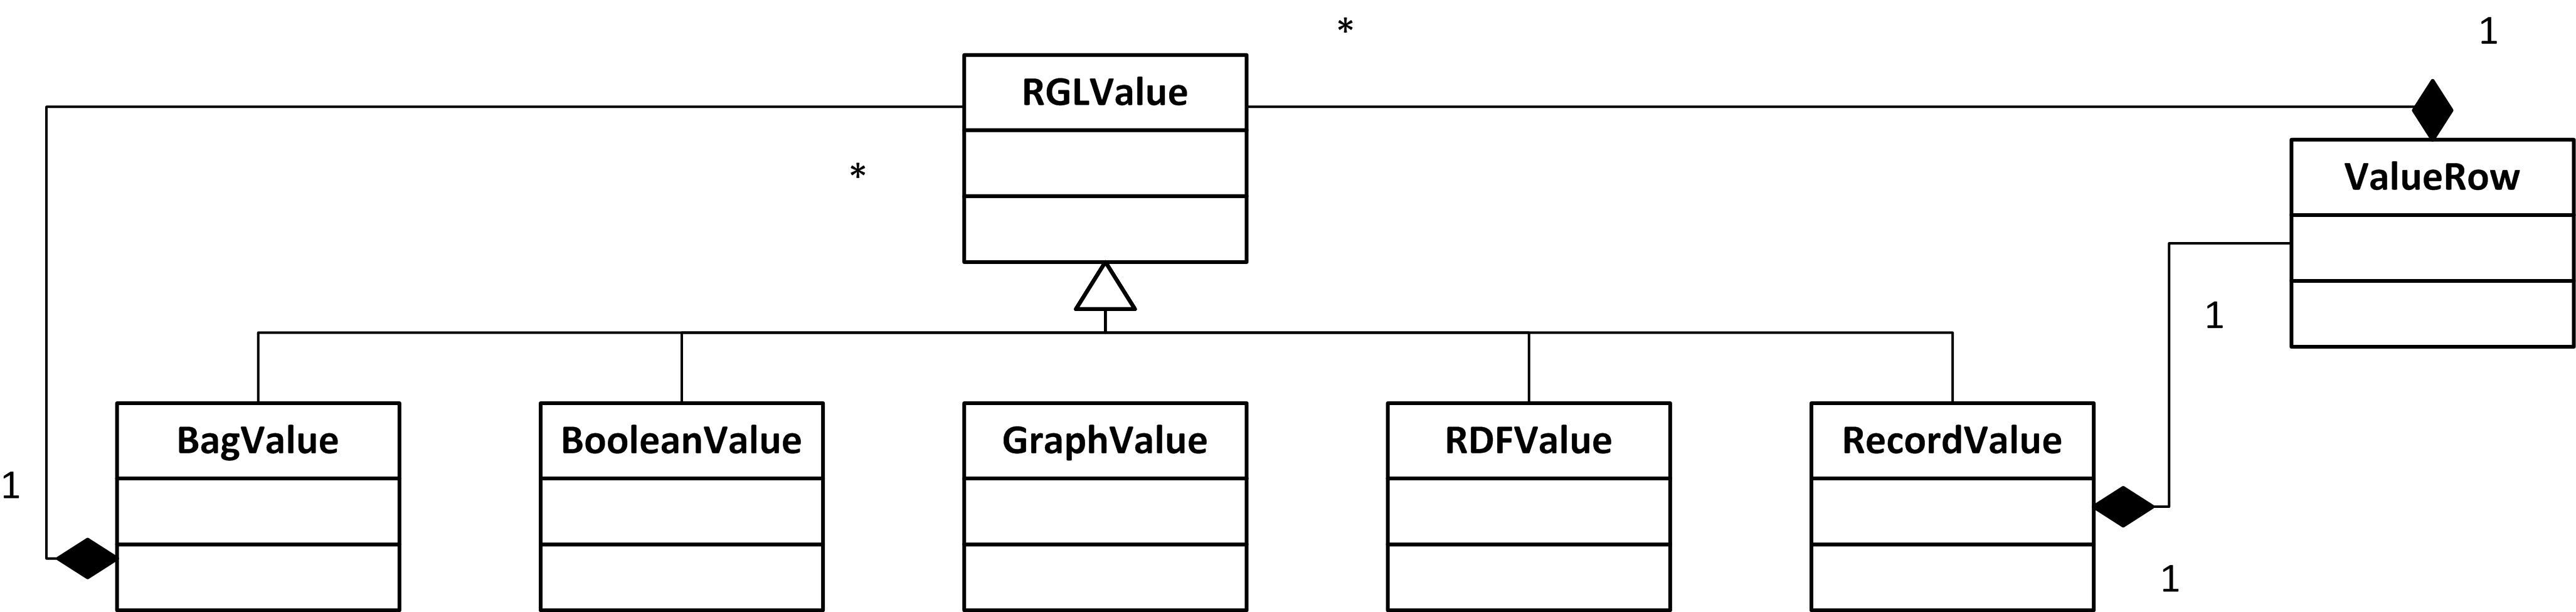
\includegraphics[scale=0.8]{diagrams/RGLValues.png}
  \caption{RGL Values }
  \label{fig_rglValues}
\end{figure}

\begin{itemize}
	\item all data is in just several tables. This is inefficient and hard to scale.
	\item entities do not have names and they are hard to locate and query
	\item structure of the data/queries is not enforced and has to be explicitly validated
	\item changing structure may leave the db in inconsistent state
	\item hard to apply access control
	\item locks and transactions
\end{itemize}

The alternative approach that we propose is to map each entity into separate JPA entity which is named after the name of the entity(has to be unique). Table \textbf{tbl} proposes a methodology to map RGL values to JPA entities. \textbf{In JPA the root element has to be entity}

\begin{center}
    \begin{tabular}{ | l | l |}
    \hline
    RGL & JPA  \\ \hline
    RecordValue/ValueRow & class (with properties)  \\ \hline
    BagValue & bag  \\ \hline
    BooleanValue & Property of type boolean  \\ \hline
    RDFValue & Property of type string  \\ \hline
	GraphValue & Property of type string  \\ \hline
    \end{tabular}
\end{center}

This approach does not suffer from the problems of the first approach. However, it exposes several issues. The first thing is that each time the structure of an entity changes the JPA mapping and the schema of the underling db has to be changed. Our solution to this problem is discussed in the next section. The second thing is that JPA requires that each entity has distinct id but RGL does not provide such properties. We solve that problem by introducing auto generated ids for each entity which are made transparent to the client system(RDF Gears). Finally, entities must have distinct names. We solve this problem by making sure that each user defined entity has a unique name, and all record properties have distinct names. In order to make the names of sub-entities(records) distinct we append to the front of their name the full path from the root entity separated by "\_".


\subsubsection{Entities are virtual}
Once we know how to map the RGL entities to JPA entities we should enable jpa to deal with this RGL entities. However, JPA expects that each entity will have its own class representing it but our entities are virtual and are no java classes that represent them. One solution to this problem would be to generate this classes on runtime. However, this approach is complex and error prone. Therefore, we continued our research for simpler approach. We discovered a promising feature in hibernate called "Dynamic models". It basically allows to define the orm logic into a mapping xml file and in run time present the data as java collections(Maps, Lists, Sets, etc.)\textbf{tbl RGL to collection}. Therefore, when an entity is defined we have to build the xml mapping file and on runtime convert the rgl entities into java collections and use jpa to store them into the database.

\begin{center}
    \begin{tabular}{ | l | l |}
    \hline
    RGL & Java  \\ \hline
    RecordValue/ValueRow & Map  \\ \hline
    BagValue & List  \\ \hline
    BooleanValue & boolean  \\ \hline
    RDFValue & String  \\ \hline
	GraphValue & String  \\ \hline

    \end{tabular}
\end{center}
 
\subsubsection{Entities are dynamic}
\textbf{Discus no-sql vs sql}
The problem that has to be solved concerns the dynamic nature of the entities. In our solutions we want to enable users to update them if this is required. Unfortunately, ORM frameworks are not good in dealing with such things. The problem is that whenever the structure changes not only the mapping xml file has to change but also the database schema. Some JPA providers provide simple tools for table generation problem(e.g. hibernate's hibernate.hbm2ddl.auto option) but they are not applicable(recreate the entire db) or not recommended in production mode(update). Therefore, in order to solve that problem reliably our solution provides implementation that is responsible to first update the mapping files and secondly update the structure of the database using JDBC statements.

\begin{center}
    \begin{tabular}{ | l | l |}
    \hline
    JPA & SQL  \\ \hline
    Class & Table( + fk to owner ) \\ \hline
    BagValue & -  \\ \hline
    BooleanValue & Column of type boolean  \\ \hline
    RDFValue & Column of type VARCHAR  \\ \hline
	GraphValue & Column of type VARCHAR  \\ \hline
    \end{tabular}
\end{center}

\subsubsection{Operations}
We have to identify how each of the CRUD operations is performed. The solution provides a RDF Gears component that is responsible to enable the user to configure and execute each type of the supported operations and convert RGL to JPA and vice versa.
\begin{itemize}
	\item create - this is operations inserts and entity into the database. The user has to provide the name of the entity that has to be stored and the data itself.
	\item read - JPA provides a special high level query language which ommits details about the internal representation of the stored data. Because of the direct mapping from rgl to jpa all possible operation on the predifiened entities makes sense. The only exception are the additional id field. In order to make it transparent to the users we will name it "\$id\$"(hibernate uses this notation to identify service fields) and using this field in queries will be forbidden.
	\item delete - normally in jpa is based on id, but since we do not have this in the semantics we provide an alternative approach. In this case users write a read query and all results(entities or sub entities) from the query are deleted. Users are responsible to make sure that the query will produce only the needed results
	\item update - like delete, update in jpa is also based on ids. So we approach the problem similarly the user writes a query that selects all entities(sub entities ) that will be updated. However, here we distinct two types of updates. The first one is to replace the value of a field(simple type, record or bag). The second one is responsible to add element into a bag.
\end{itemize}

\subsection{Multitenancy - How to enable multiple users to use the solution and collaborate?}
The second main challenges that we have to solve is to enable multiple users to work with the solution simultaneously. In literature this is referred to as multi-tenancy. It has significantly increased its popularity in recent years as a results of the advancements in cloud computing and database as a service in particular \cite{Hui}. 

Designing the solution we have to take into account the following things: how to organize the data into the database, how to enable collaboration and how to manage access control.

\paragraph{Database organization}
There are three main approaches for designing multi-tennant solution \cite{Hui}:

\begin{itemize}
	\item \textit{Independent Databases and Independent Database Instances (IDII)} - in this approach users share only the hardware(server). For each user an independent database instance is running. This approach provides good data isolation and security but maintenance cost is significantly increased as a result of the multiple running instances. Additionally, collaboration between engineers is problematic because of the difficulty to execute queries on data that is spread over several databases.  
	
	\item \textit{Independent Tables and Shared Database Instances (ITSI)} - in this approach users share the hardware but also the database instance. Each user has private tables(user id is usually appended at the beginning of the table name \cite{Hui}). This approach reduces the maintenance cost but still the number of tables increases linearly with the number of users. Collaboration is facilitated but querying data relating all users he has to union the data from all user tables. Another disadvantage of this approach is that because the tables are different for each user we also need a separate JPA mapping for each user with increases complexity additionally.
	
	\item \textit{Shared Tables and Shared Database Instances (STSI)} - in this approach, all users share the db instances as well as the tables. In this approach the number of tables does not increase when the number of users increase. As a result the maintenance cost is reduced, queering is simplified(no unions required) and JPA mapping is straight forward. However, this approach has some disadvantages. First, engineers are responsible to maintain the required level of isolation between different users(usually a column indicating the owner of the data is required and additional where clause when querying for particular user). Second, tables contain the data for all users which may lead to decrease of performance.
	
\end{itemize}

Discussing the advantages and disadvantages of all the approaches above, we decided to use the STSI because it is easy to map to JPA, enables collaboration, simplifies querying and is easier to maintain.    

\paragraph{Collaboration}
The ability for engineers building workflows to collaborate and reuse each others data is essential \cite{Lu}. Choosing STSI organization makes it easy for engineers to work with the data of the others. However, there are several issues that has to be discussed and addressed:

\begin{itemize}

	\item \textit{privacy} - sometimes users might not want others to use their data. This might be because of a privacy issues or entities are not designed to be shared. Additionally, engineers might want to limit the access to the data. For example they might only allow others to read the data but not to modify it. Therefore, when the engineer defines an entity he should be able to specify its sharing options which are enforced by the solution.
	 
	\item \textit{semantics and structure of shared data} - the solution can further assist engineers that want to reuse shared data by providing information about its structure and semantics. Implementing such functionality will save them a lot of time since otherwise this information has to be communicate by other means which may take a lot of time.
	
	\item \textit{entities mutation} - introducing the multi tenancy feature introduces the problem with the consistency. By design entities can change and evolve over time. Therefore the system should prevent any inconsistent results produced if the structure changes at the time a workflow is executed. Our solution deals with that problem using transactions. All data operations are executed in transactions which temporary lock the tables for modification. As a result, the changing request will wait for the tables to be released before applying the updates to the database schema.
\end{itemize}


\paragraph{Access control}

The solution has to be able to enforce the sharing options of the entities and make sure that data is not accessed illegally. Therefore, the solution provides access control functionality that is responsible to enforce this policies. Basically, jpa is not good at doing this, it does not provide any access control functionality out of the box(\textbf{check that}). Therefore, there are two possible places to put the access control logic. 

\begin{itemize}
	\item \textit{above JPA} - our solution wraps arround the JPA engine and thus, we can control all the requests that it receives. We can provide functionality that validates if the user has the needed permissions to execute that functionality. However, from engineering perspective doing this will be hard since JPA(JPQL) allowes engineers to consrtuct relatively complex queries and building a functionality that pareses this queries is not a trivial job to do which significantly increases the risk of security wholes.
	
	\item \textit{underling DB} - the second option is to make the database enforce the security policies. We think that this approach is much easier because database already provide sophisticated fine grained access control mechanisms(\textbf{cite needed}). The only think that we have do is to translate the security policy of our solution to the database language(DDL) and set them when an entity is created or modified. As a result, the database will stop the JPA accessing data that it is not authorised to access.
\end{itemize}

\subsection{RDFGears extension - How to enable RDFGears to work with this new kind of functionality?}
what are side effects

To understand the problem this new components introduce we first have to understand how RDFGears work. 
how rdfgears works

rdfgears does not have any or branching and therefore it is expected that all components are executed. However, in order to improve efficiency it introduces some optimizations:
\begin{itemize}
	\item the engine compiles the workflow into a datastructure which contains the output node and all components that the output directly or indirectly depends on. Therefore, components that do not have (indirect) connection to the output node are omitted. This makes sense because the assumption is that components do not have any side effects and if they do not contribute for the final result then there is no difference if they are executed or not.
	
	\item the engine takes the output node and recursively executes all components which outputs are needed for the execution.
	  
	\item the results produced by a component are cached. Therefore, if their output is needed in several branches the value is calculated only once.
	
	\item iterations ...  
\end{itemize}

The problem is that our solution imposes on this optimizations is that the assumption that components do not have side affects is no longer correct. Therefore, the engine will not longer perform its tasks correctly. The trivial approach would be to simply remove all these optimizations but this is not a good idea because efficiency will suffer continuously. Therefore, we propose an alternative approach which aims to make the engine perform correctly but also keep the efficiency.

Our solution consists of the following steps:
\begin{itemize}
	\item extend the function description notation so that the engine knows if a component has side effects or not
	\item when the datastcutrure of the functions is built we also include the components that have side effects and recusivly all the components that they depend on.
	\item we perform all the optimizations to the output node(as it is currently done) as well as to all components with side effects. 
	\item when the workflow is executed we execute it for the output node and for all components with side effects. The caching mechanism prevents components to execute several times. The output of the workflow is still the output of the output node.
\end{itemize}

These steps ensure that all components with side effects are executed and the execution is efficient because all the optimizations are applied.

\subsection{Integration with the plugin environment}

We implemented an additional special feature that aims to save save time to engineers. The idea of this feature is to integrate the datamanagement feature with the plugin environment feature. The benefit from this feature covers the situation when engineers create a certain kind of user modeleing service which requires data interactions and  bundle it into plug-in. Since this feature interacts with data if will most probably require entity deffinitions is order to work. Therefore, every time this plug-in is deployed on a server the engineers has to manually define the needed entities through the user interface. Obviously, this operation may cost signlificant time and is error prone. Additionally, the problem becomes severe when an engineers wants to use a shared plug-in produced by someone else. In this case the two engineers need a way to somehow exchange the entity definitions.

In order to solve that problem we have devised a mechanism that can deal with this issue automatically and thus safe time to the engineers. The idea is very simple. Each entity definition is stored in an xml file in the file system. Therefore, the first time an engineers creates an entity definition it can export it as an xml file. Then, he can include this file in the plugin and register in in the \textbf{plugin context}. When this plug-in is installed the system automatically detects the presense of this entities and installs them automatically so that the functionality of the plug-in can be used right away without any need for configuration.

\section{Architecture}
We have already discussed the main problems that our solution is facing and the approach we will use to solve each of them. In this chapter we discuss the architecture of the solution.

\subsection{Context View}
\textbf{po skoro ne tazi sekciq}
\begin{figure}[h!]
  \centering
  	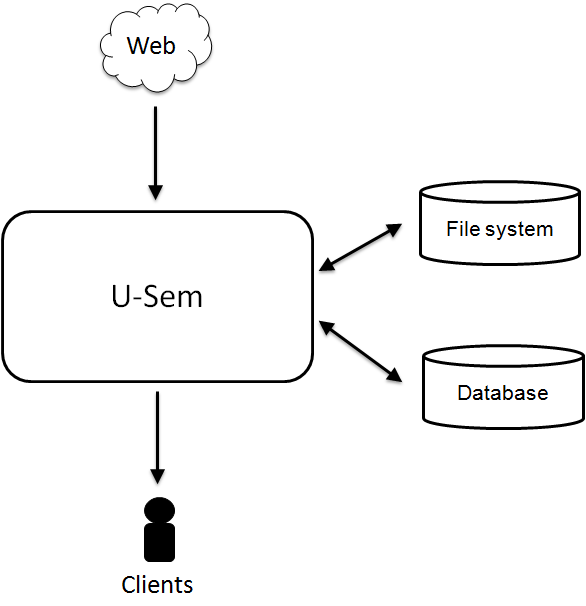
\includegraphics[scale=0.4]{environment/runtime_environment_storage.png}
  \caption{Context diagram of U-Sem }
  \label{fig_context}
\end{figure}

\subsection{Functional View}

All components that take part in the data management functionality can be classified in three layers. This organization is illustrated in figure Figure \textbf{fff} and consists of the following layers:

\begin{figure}[h!]
  \centering
  	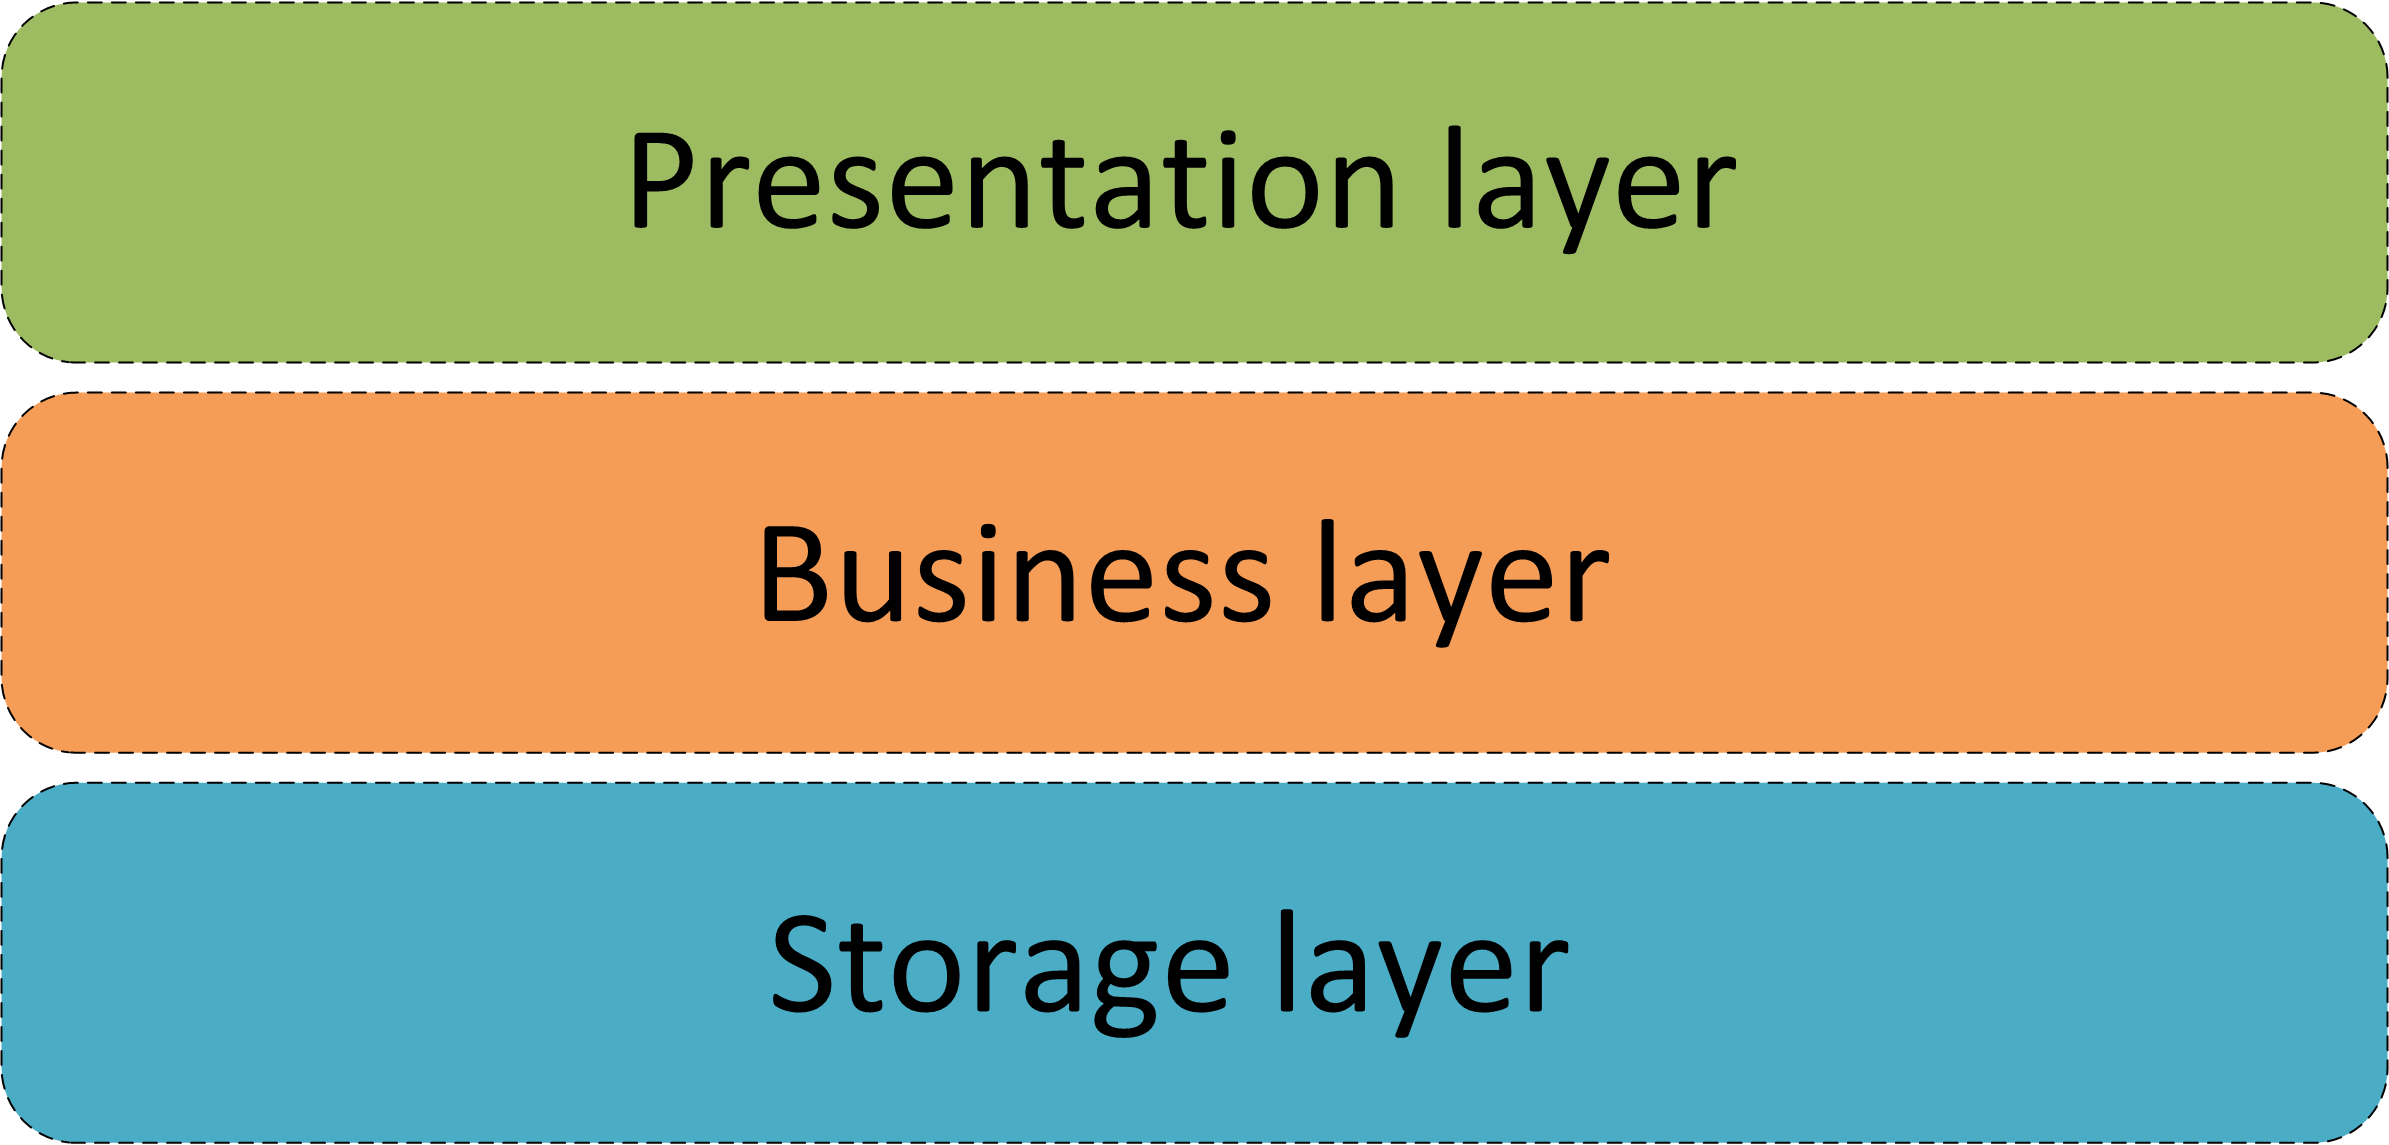
\includegraphics[scale=0.4]{functional/layers.png}
  \caption{Context diagram of U-Sem }
  \label{fig_context}
\end{figure}

\begin{itemize}
	\item \textit{Application layer} - this layer consists of all functional components that are interested in the data management feature. These applications are responsible to provide functionality to the user for defining and manipulating data.
	
	\item \textit{Business layer} provides functionality for defining the structure and semantics of the data and manipulating the actual data. The functional components that build this layer are responsible to enforce the security and privacy policies of the system.
	
	\item \textit{Storage layer } is responsible to provide storage functionality for storing the entity definitions, the hibernate mappings and the actual data.
\end{itemize}

\subsection{High-level component organization}
This section describes the internal structure of the layers and identifies the high level components that build up the feature. Figure \textbf{3.11 ffff} illustrates this organization. It shows how the high-level components are organized into the layers and the way they depend on each other. We have identified the following high level components:

\begin{figure}[h!]
  \centering
  	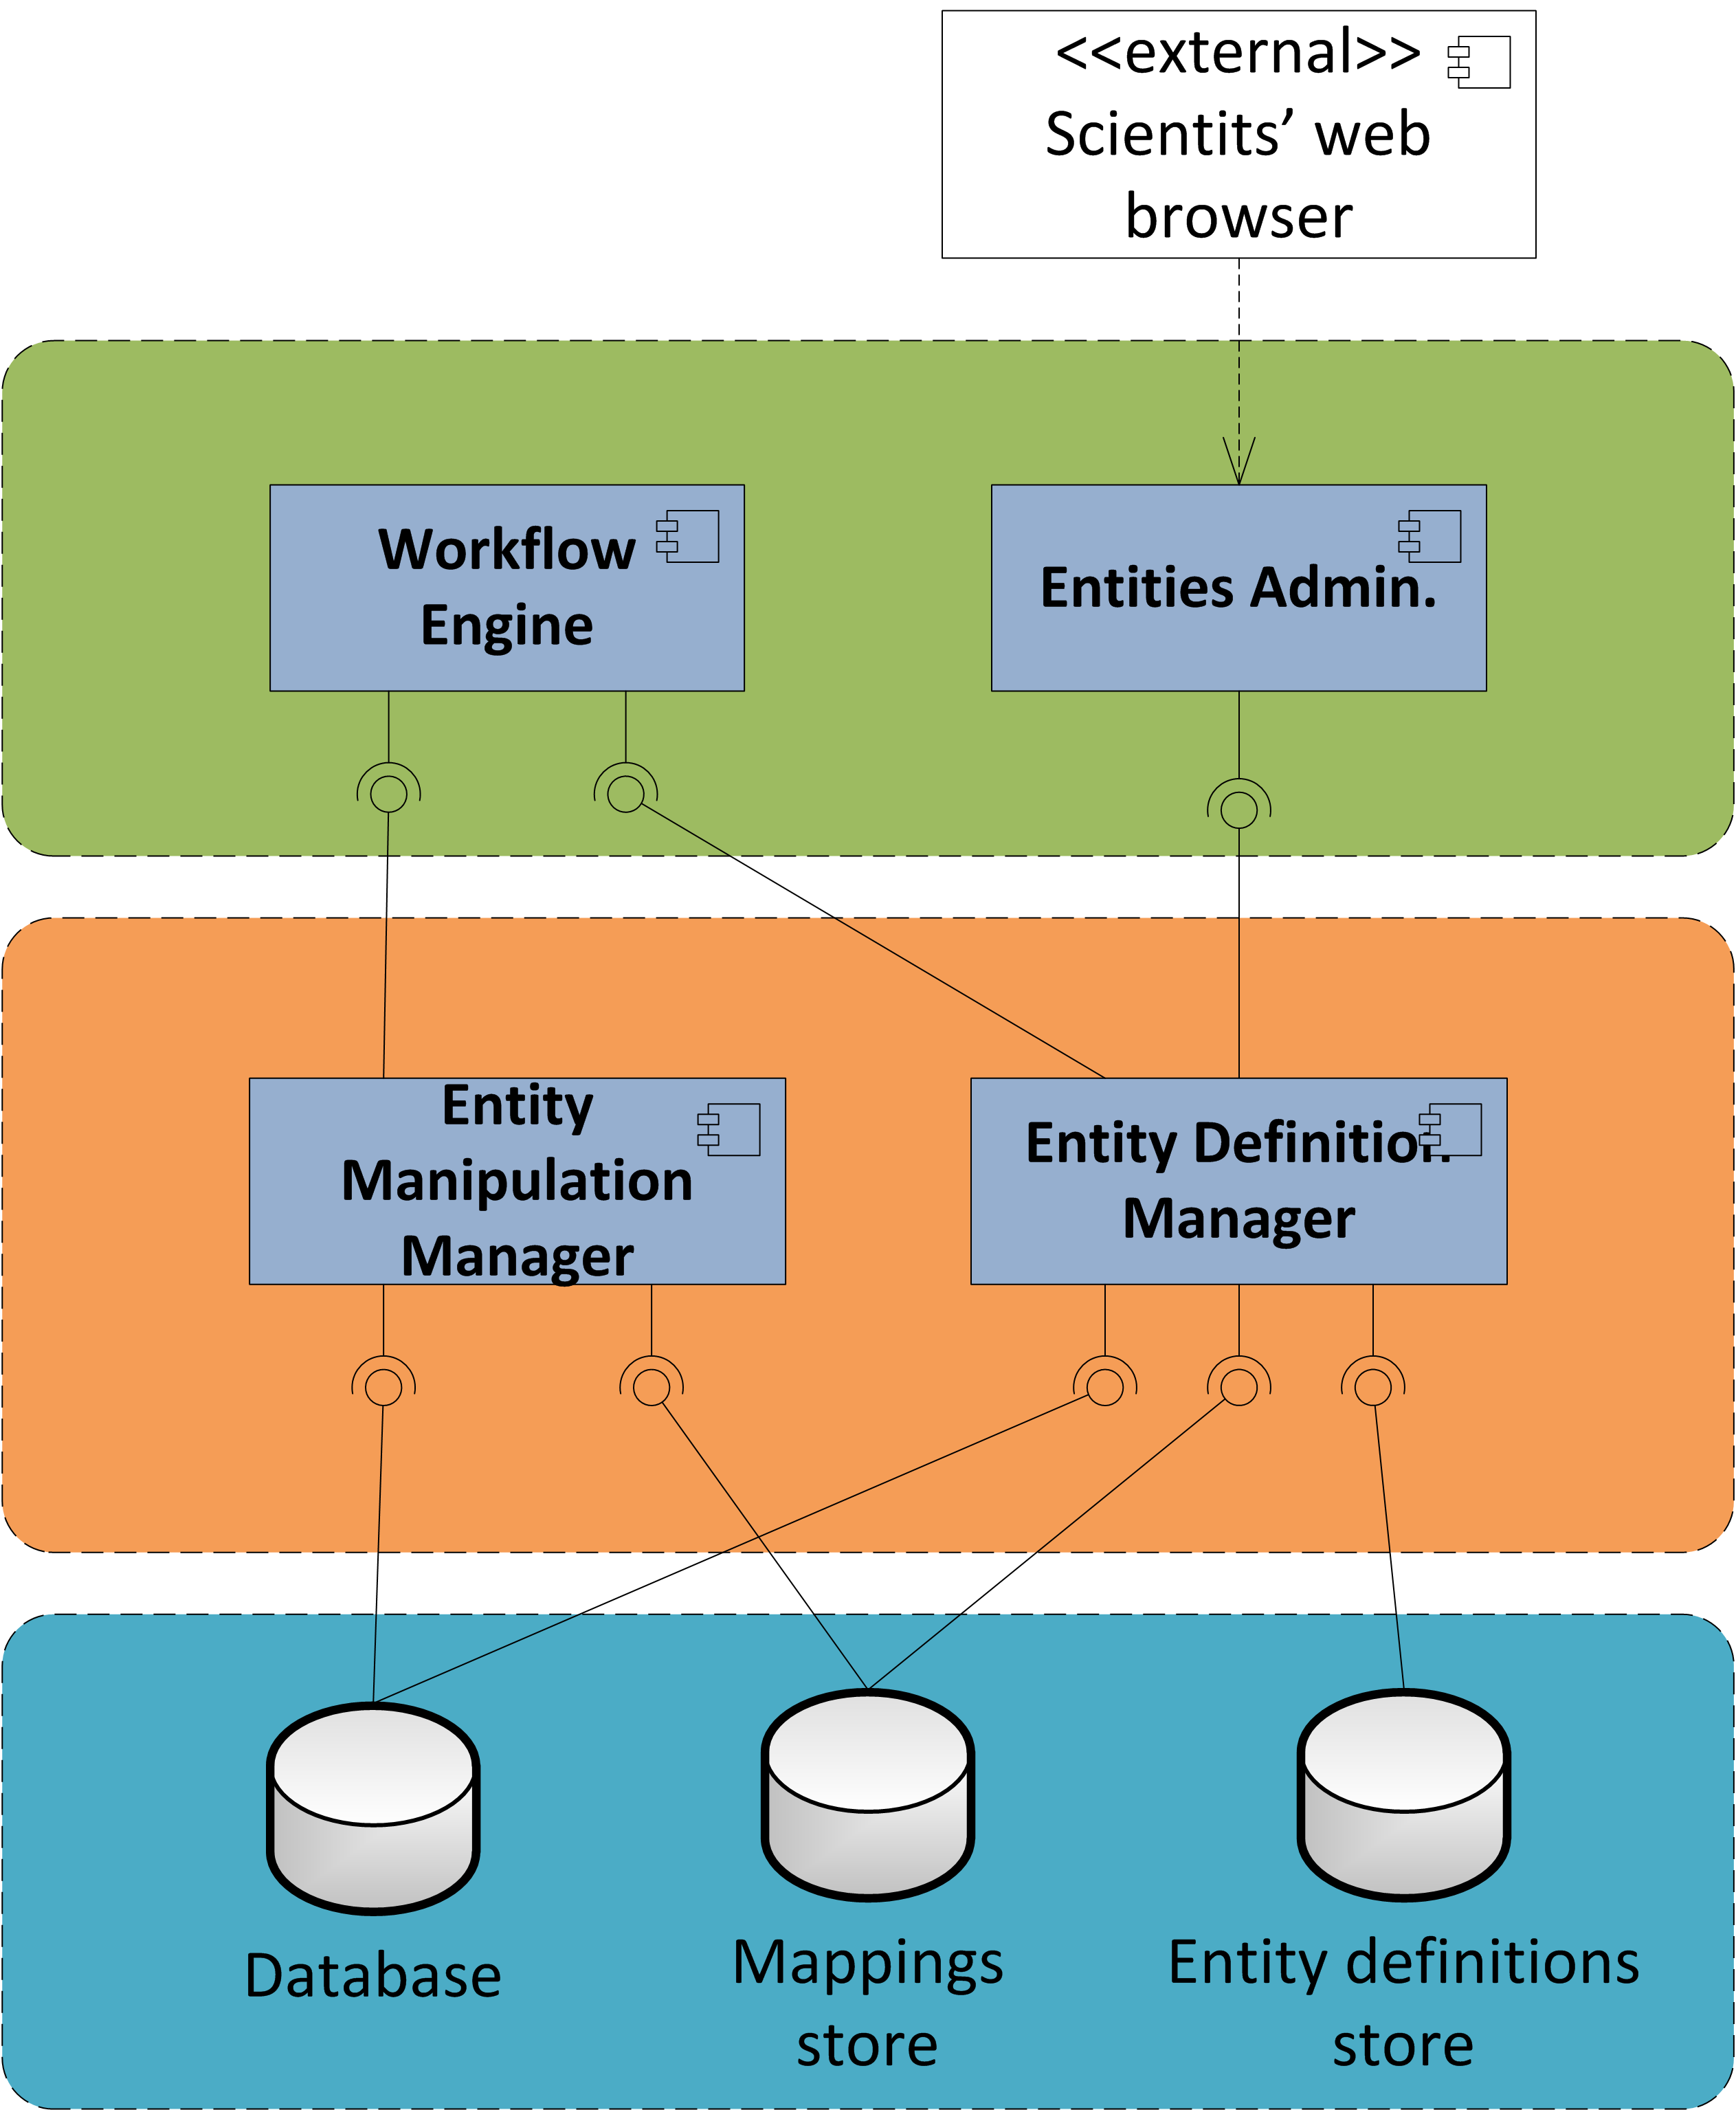
\includegraphics[scale=0.6]{functional/func_main.png}
  \caption{Context diagram of U-Sem }
  \label{fig_context}
\end{figure}

\begin{itemize}
	
		\item \textit{Entity definitions store} - Provides functionality for storing the data describing the entity definitions. 
		
	\item \textit{Mappings store} - Provides functionality for storing the data defining how entities are mapped to the database.  
	
	\item \textit{Database} - SQL database that stores the actual data.
	
	\item \textit{Entity Definition Manager} - this component is responsible to provide the logic for defining the structure and the semantics of the data entities. It is also responsible to provide the mappings that state how the data is mapped to the database. Additionally, this component is responsible to prepare the database(create SQL tables and set access permissions) for working with the defined entities. The functionality is exposed by a API that enables the high level components to manipulate the entity definitions. Further decomposition of this component is provided in the next section.
		
	\item \textit{Entity Manipulation Manager} - this component is responsible to provide the functionality needed for manipulating the data based on the previously defined structure(entity definitions). It provides implementation for creating, updating, deleting and querying data. It is also responsible to enforce the access control over the data. High level components access the functionality provided by this component through an API. Further decomposition of this component is provided in the next section.
	
	\item \textit{Entities Admin.} - is responsible to deal with the administration of the data entities. It provides the system`s endpoint(user interface) for interaction with the scientists. Further decomposition of this component is provided in the next section.

	\item \textit{Workflow Engine} - uses the interface provided by the Entity Definition Manager and Entity Definition Manager to enable engineers define data entities and create services that manipulate persistent data. During the workflow configuration phase it uses the entity manipulation interface in order to obtain the list of already defined entities(their structure and their semantics) assisting the user to easily define workflows that require data manipulation. During the workflow execution phase it uses the Entity Manipulation interface to execute the defined data operations.
\end{itemize}

\subsection{Entities administration}
This section defines the functional decomposition of the Entities administration component which is illustrated on figure \textbf{fff}. It consists of the following components:

\begin{figure}[h!]
  \centering
  	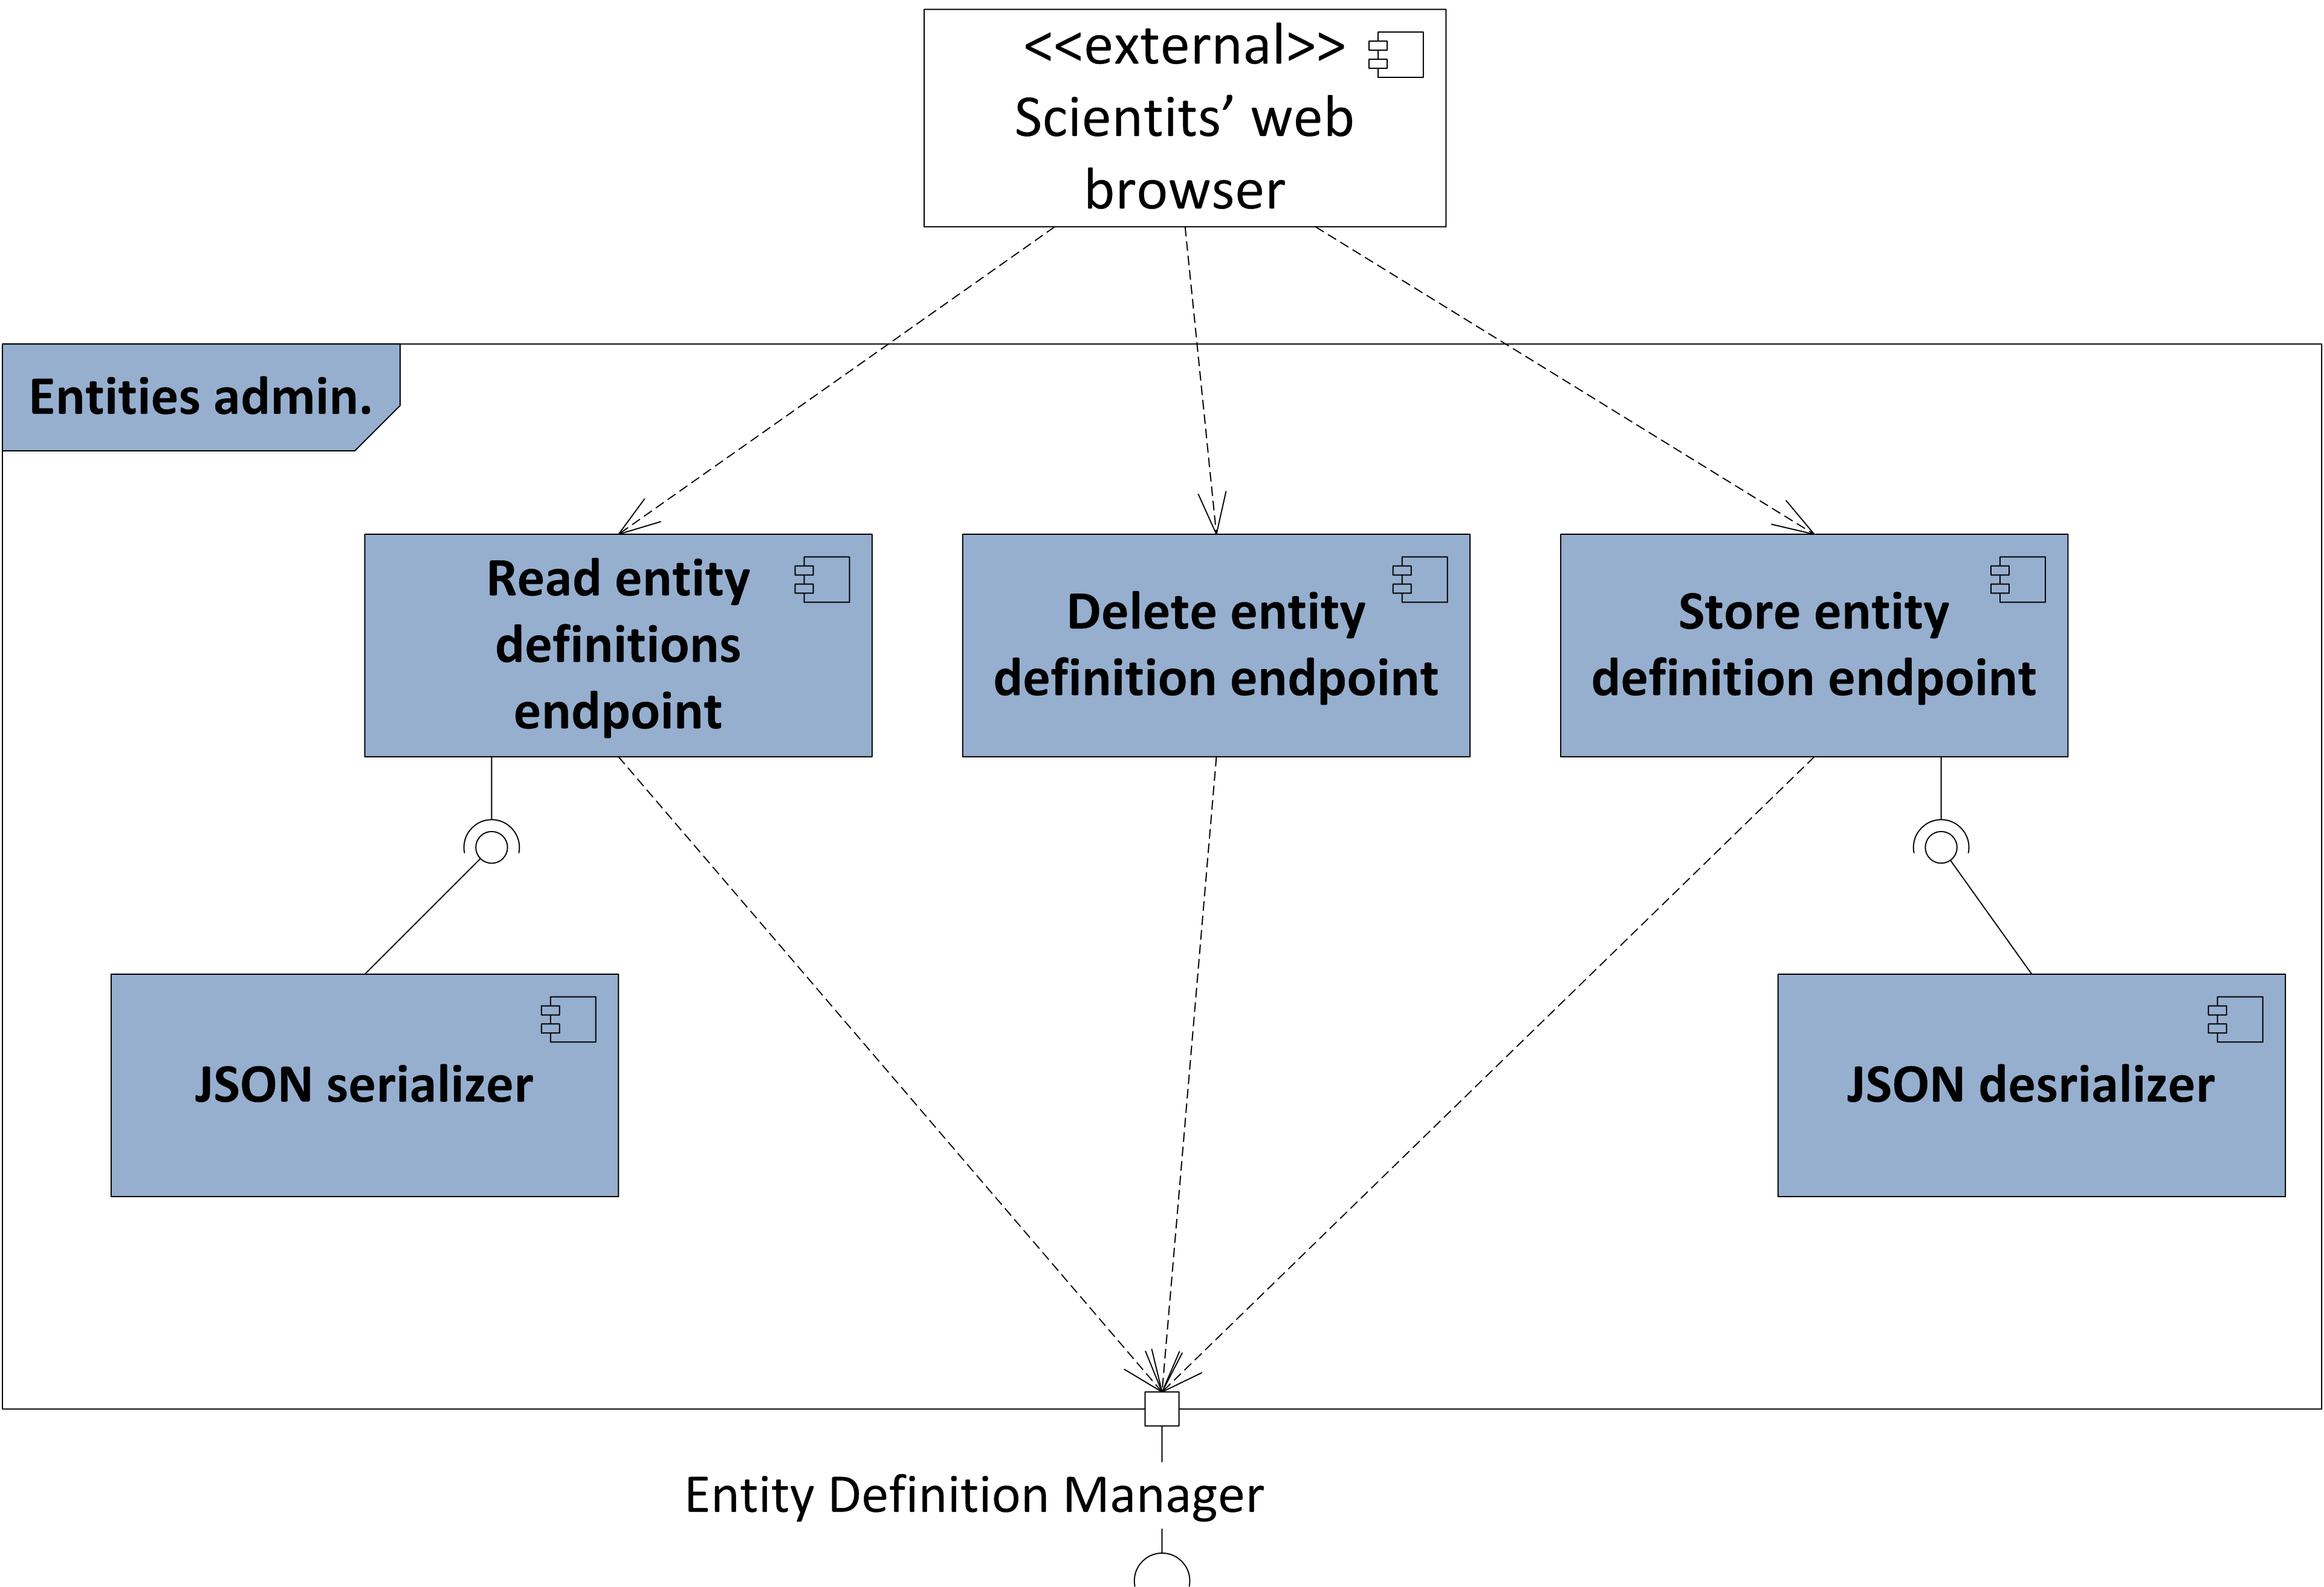
\includegraphics[scale=0.6]{functional/func_admin.png}
  \caption{Context diagram of U-Sem }
  \label{fig_context}
\end{figure}

\begin{itemize}
	\item \textit{Read entity definitions endpoint} - This component provides the user interface needed for browsing the already defined entities.
	
	\item \textit{Delete entity definition endpoint} - This component provides the user interface needed for removing a selected entity.
	 
	\item \textit{Store entity definition endpoint} - This component provides the user interface needed for creating new or updating existing entity definition.
	
	\item \textit{JSON de/serializer} - Since data in the user interface is presented in the form of JSON. This component is responsible to convert the entity definitions from/to JSON format.
	
\end{itemize}

\subsection{Entity Definition Manager}
This component is responsible to provide API which can be used by application layer components in order to manage the entity definitions. Figure \textbf{fff} shows the functional decomposition of the \textbf{Plug-in access manager} module. It consists of the following components:

\begin{figure}[h!]
  \centering
  	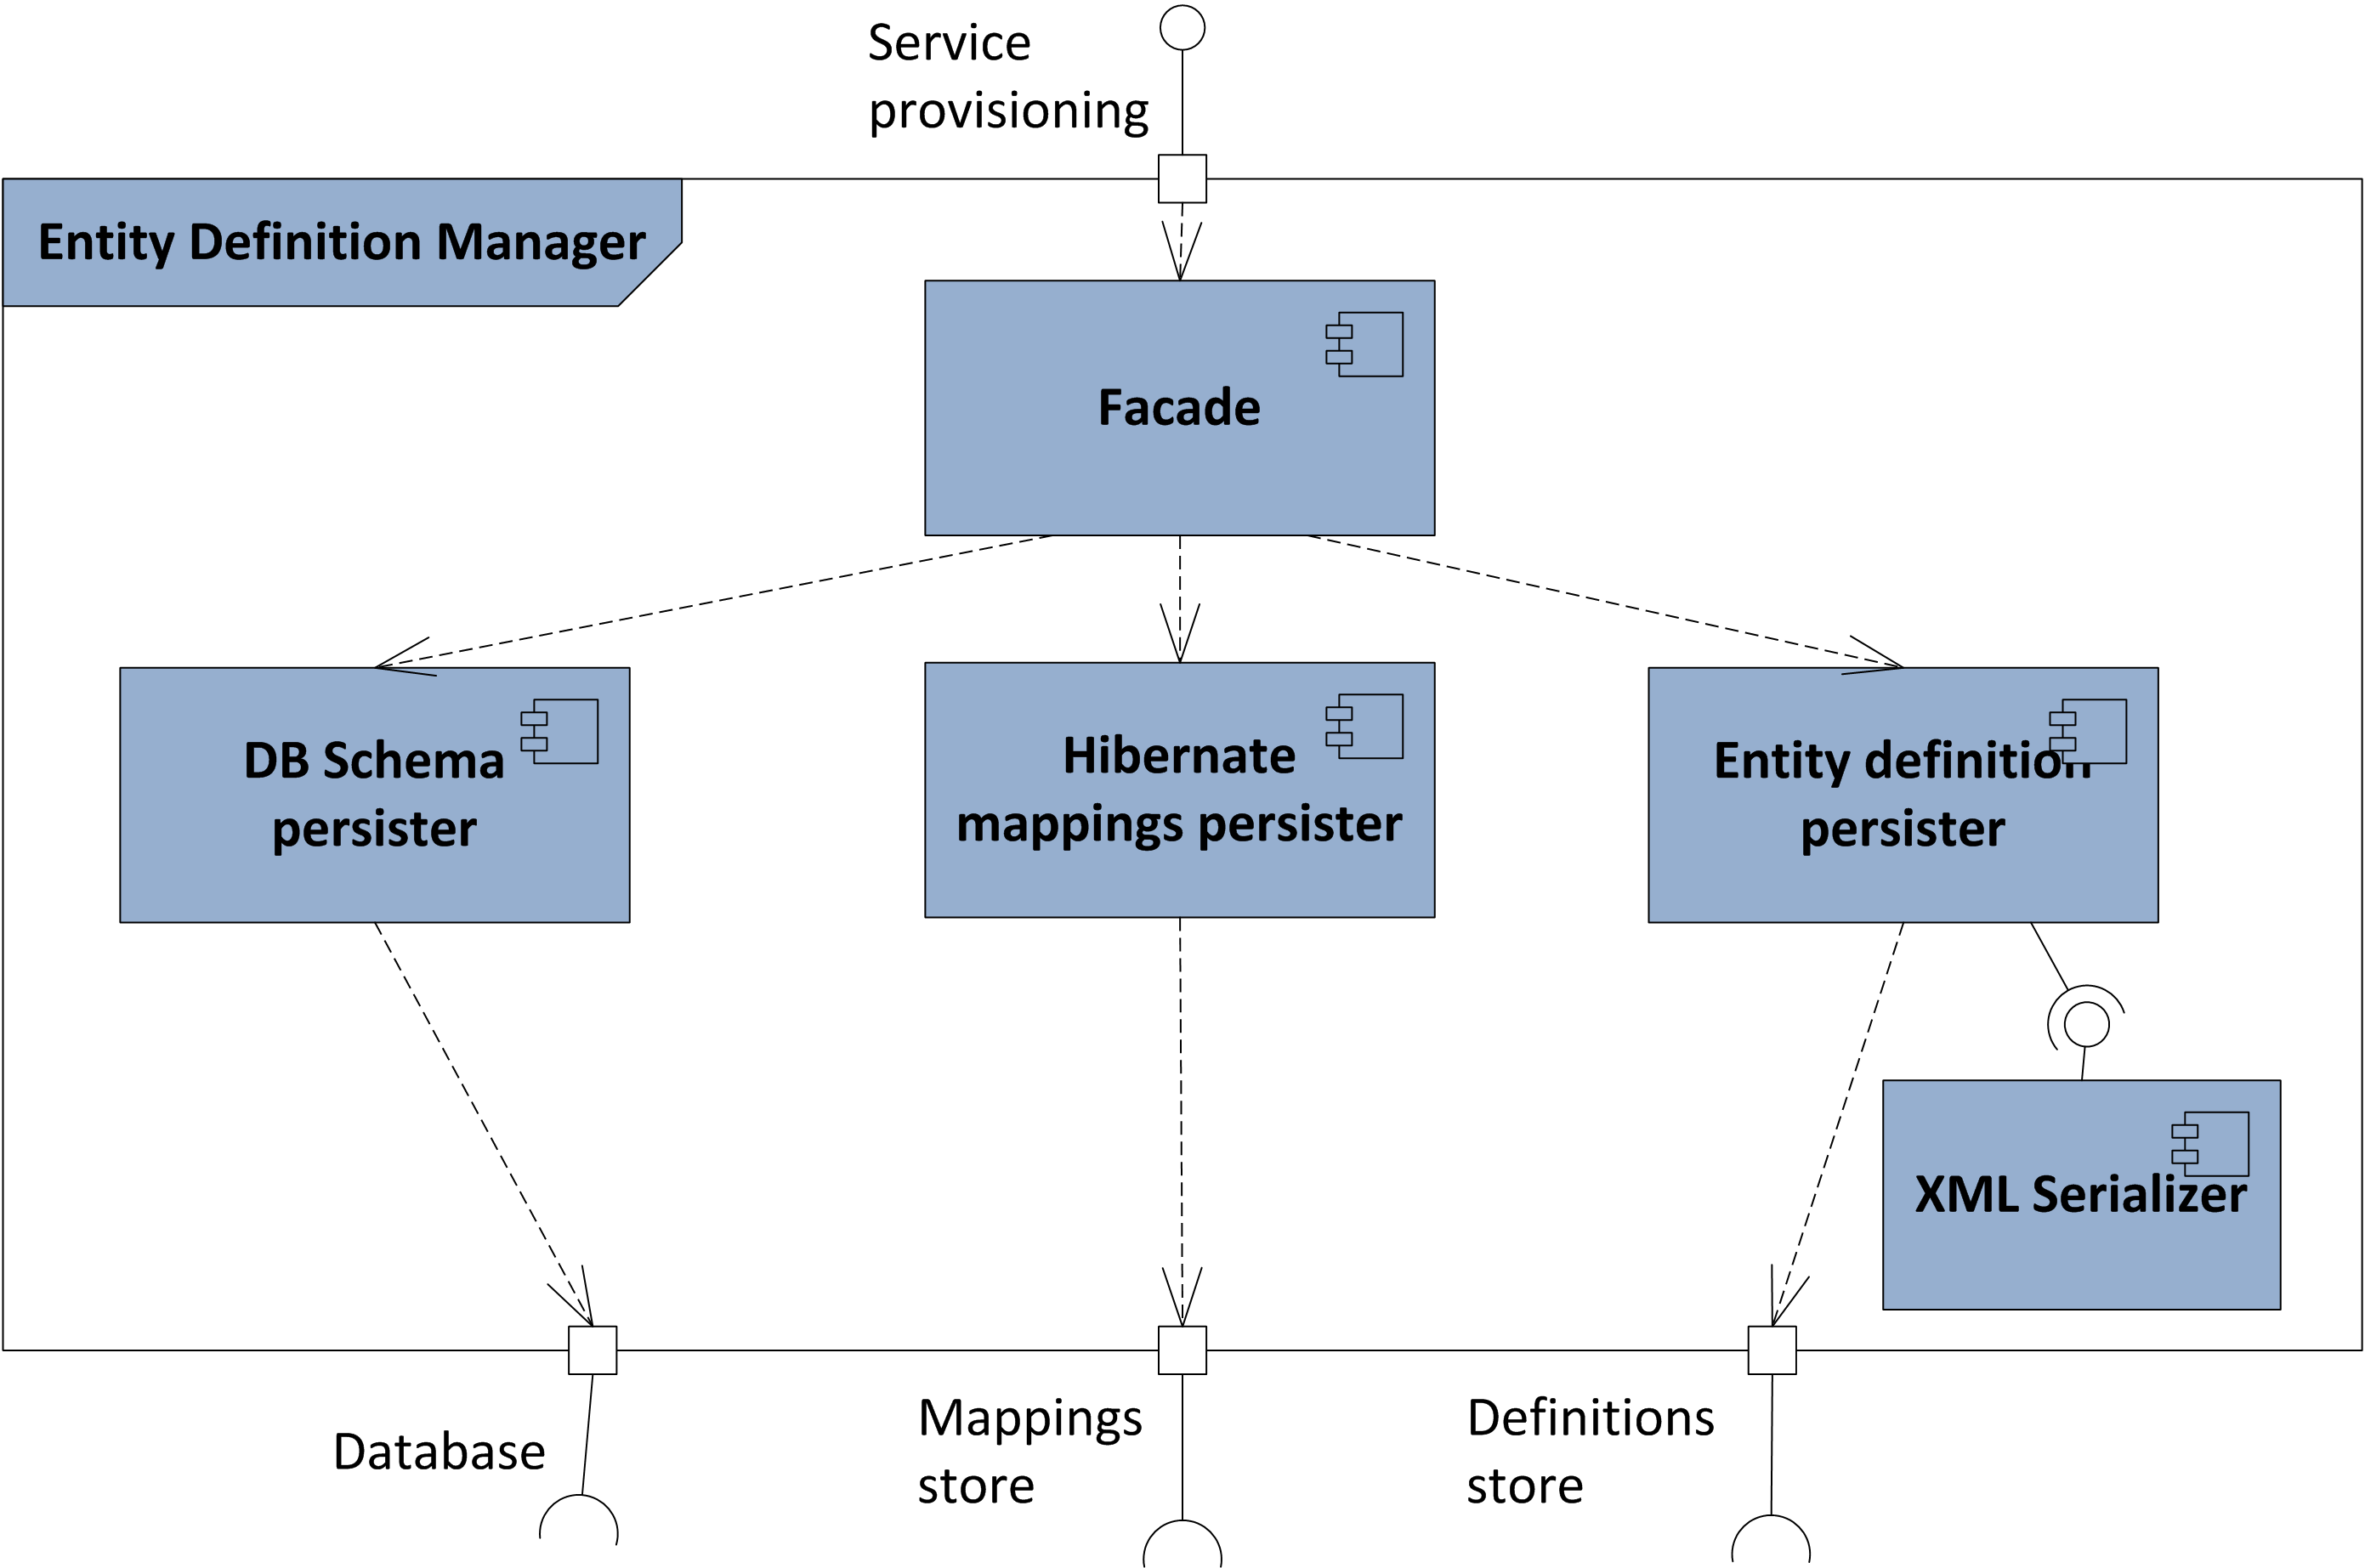
\includegraphics[scale=0.7]{functional/func_access.png}
  \caption{Context diagram of U-Sem }
  \label{fig_context}
\end{figure}

\begin{itemize}
	\item \textit{Facade} - this component provides the API for manipulating the entity definitions.
	
	\item \textit{DB Schema persister} - this component is responsible to make sure the database schema is always corresponding to the entity definitions. Any time the entities are changed the database schema is updated. Additionally, this component also defines the access permissions for each access table based on what the user creating the entity has specified.
	
	\item \textit{Hibernate mappings persister} - this component is responsible to construct the mappings that define how data is mapped and stored in the database. Since we are using Hibernate, this information is created and stored as .hbm files.Any time the entities are changed the mappings are updated.
	
	\item \textit{Entity definition persister} - this component provides functionality for storing the entity definitions.
	
	\item \textit{XML Serializer} -  This component is responsible to store and retrieve the entity definitions. It provide a level of abstraction over the way the definitions are stored. As a result, this will be the only component that is affected in case of any change of the place and format of the data is required. The default implementation of this component stores the entity definition in the file system as xml files.
\end{itemize}

\subsection{Entity Manipulation Manager}

This component is responsible to provide API which can be used by application layer components in order to perform CRUD operations over the already defined entities. Figure \textbf{fff} shows the functional decomposition of the \textbf{Entity Manipulation Manager} module. It consists of the following components:

\begin{figure}[h!]
  \centering
  	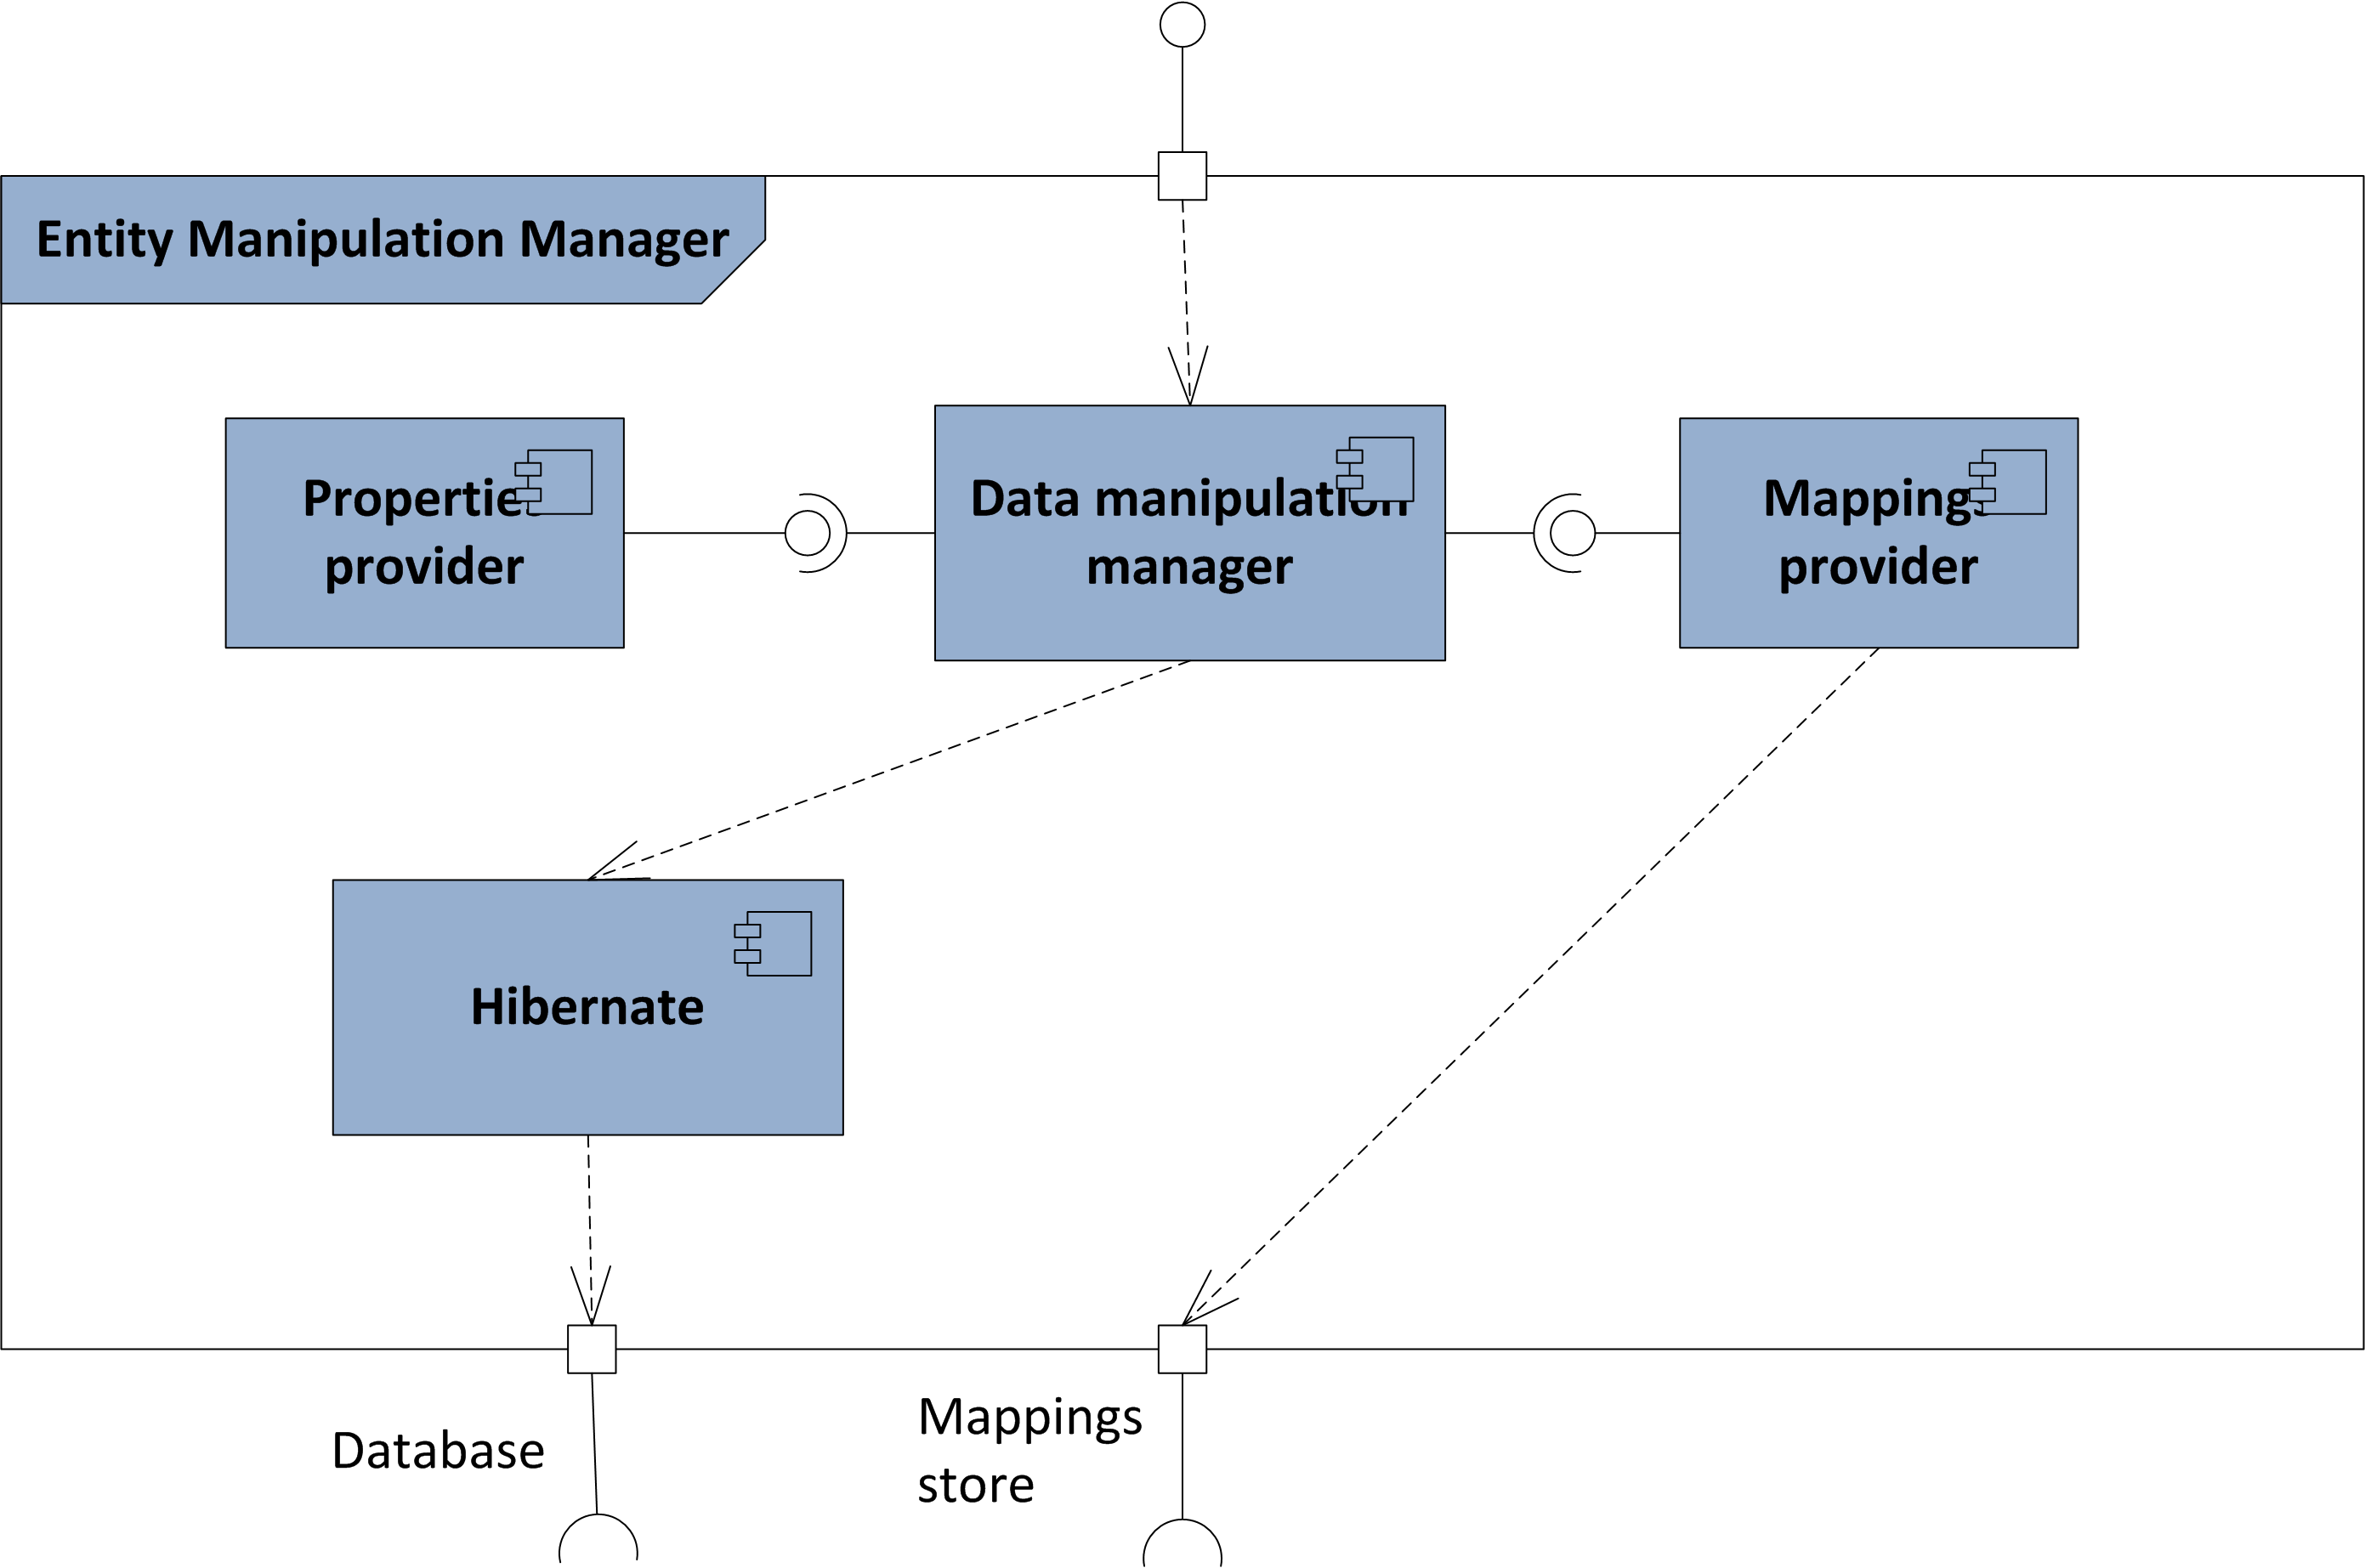
\includegraphics[scale=0.7]{functional/func_manip.png}
  \caption{Context diagram of U-Sem }
  \label{fig_context}
\end{figure}

\begin{itemize}
	\item \textit{Data manipulation manager} - this component provides the API for manipulating data. This component manages the communication with the Hibernate framework. It is responsible to start/stop the framework and monitor its life cycle. It also acts as a level of abstraction over the framework and in case any change in future is required, this will limit the number of affected components.
	
	\item \textit{Properties provider} - Keeps track of all common and user related options that are required for the correct operation of the Hibernate framework. The main properties this component is responsible to provide are the database login configuration for each user. It has to make sure that each request to the database is executed with the correct database user so that the database can handle the access control properly.
	
	\item \textit{Mappings provider} - This component is responsible to provide the "hbm" files that tell the Hibernate framework how to map the U-Sem entities(represented as java collections) to the database.
	
	\item \textit{Hibernate} - This component represents the Hibernate framework which is responsible to perform the actual interaction with the database in order to serve CRUD requests.  
\end{itemize}

\subsection{Concurrency View}
\textbf{echache problem for types}

\begin{figure}[h!]
  \centering
  	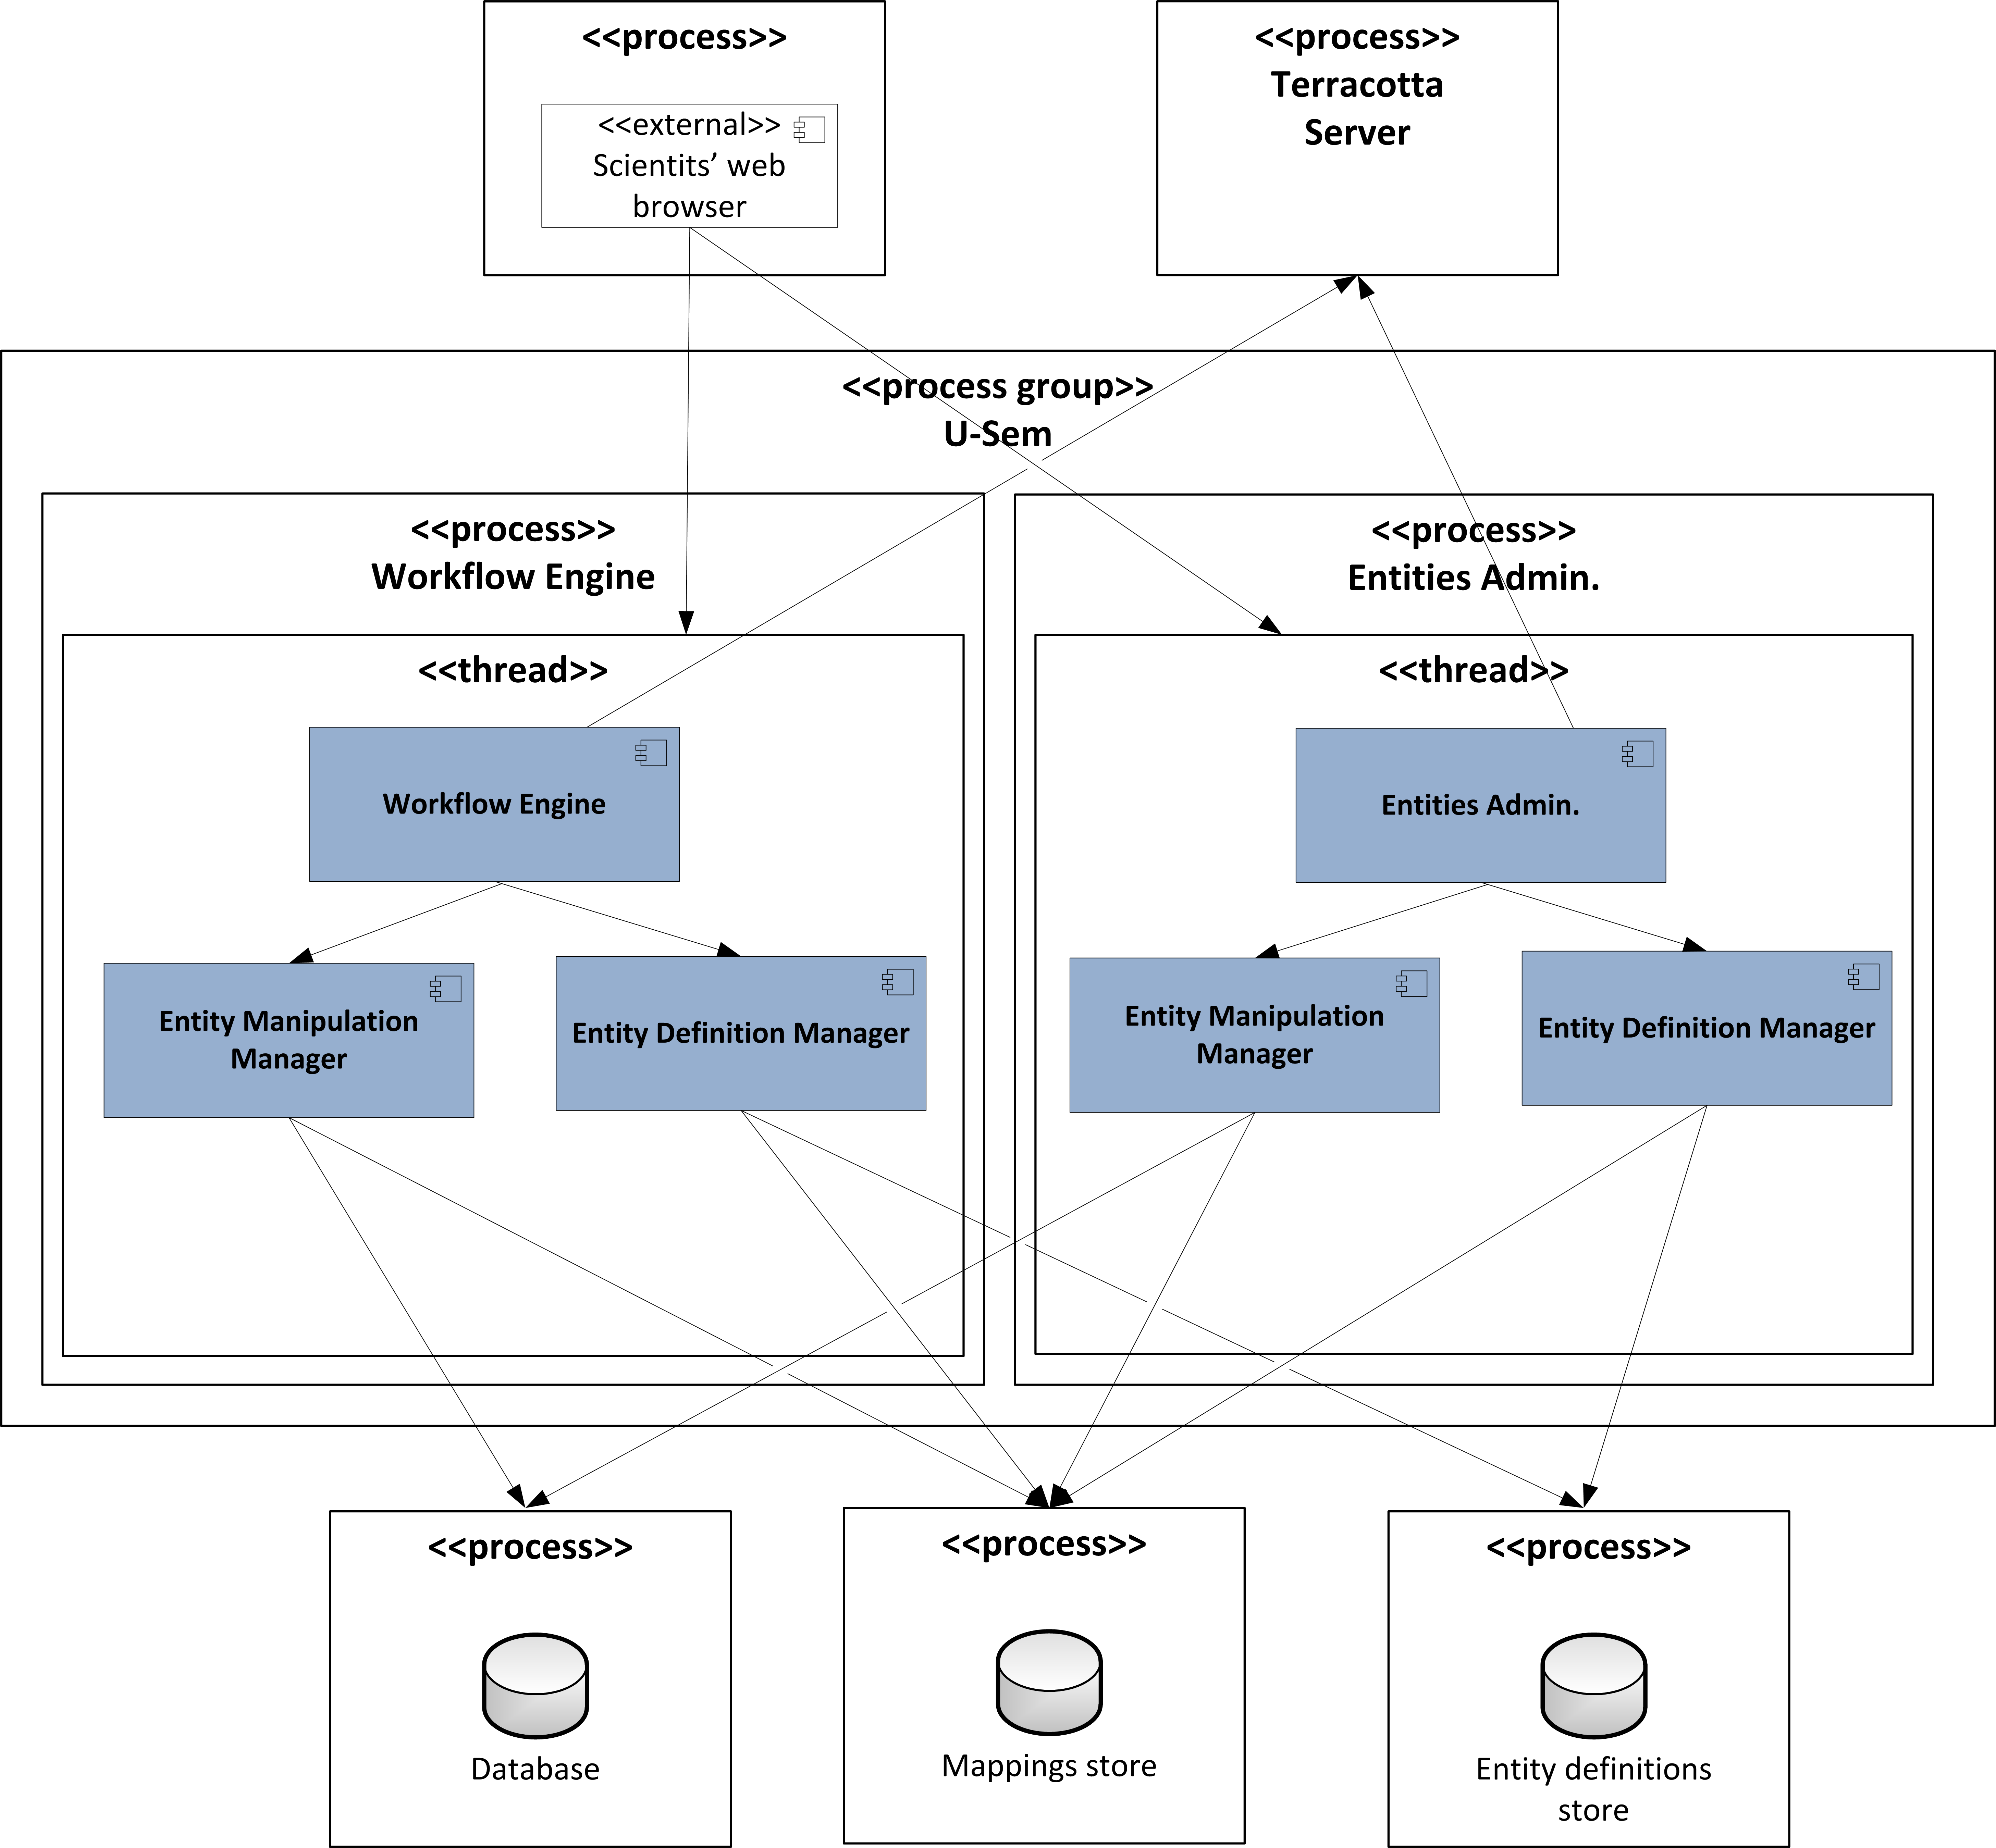
\includegraphics[scale=0.5]{functional/concur.png}
  \caption{Context diagram of U-Sem }
  \label{fig_context}
\end{figure}

This section describes the concurrency structure of the feature. We show how functional elements map to concurrency units(processes, process groups and threads) in order to clearly identify the parts of the system that can work concurrently. We also show how this parallel execution is coordinated and controlled.

Figure \textbf{fff} illustrates the concurrency organization. The main functionality of the system is situated in the U-Sem process group. All U-Sem processes including the storage processes operate concurrently. Workflow configuration and execution initiated by U-Sem clients and entity management by scientists can happen at the same time. This organization makes the solution flexible because if needed the \textbf{Workflow} process can be replicated independently from the \textbf{Administration}. However this organization also introduces some problems that has to be solved.

\subsubsection{Problems}
Firstly, if the workflow engine is the middle of execution and the structure of the database is changed, then the workflow may fail unexpectedly and cause problems that are hard to detect and reproduce. 

Secondly, every time the required resources for the data store interaction(entity definitions and mappings) are loaded the system has to make sure they are consistent with each other and also with the underling structure(schema) of the database. A problem can occur if the resources are loaded and modified simultaneously(simultaneous execution of workflows and entity definitions manipulations). It may happen that some of the files are loaded before the modification and others afterwards. This inconsistency can also lead to problems that are hard to detect and reproduce.

\subsubsection{Solution}

In order to solve the problem we propose a solution that is based on synchronization between the processes. The solution is based on the \textit{Reader-Writer Lock} idea. It extends mutual exclusion locks by enabling concurrent read access to a shared resource but requires exclusive access for write operations \cite{Lev}.

Our solution maps to the \textit{Reader-Writer Lock} idea as follows:
\begin{itemize}
	\item The shared resource is the combination of the entity definitions, mapping and the database schema.
	\item The workflow engine acts as reader of the shared resource.
	\item The entity administration acts as writer of the shared resource.
\end{itemize}
As a result, multiple workflows can be executed simultaneously but when a change to the entities is needed it is executed exclusively. Therefore, the workflow engine is protected against loading the resources while they are inconsistent.

However, the standard \textit{Reader-Writer Lock} in Java works only within the virtual machine \cite{javadocs}. In our case we have to synchronize entire processes. Our research showed that there are already tools that provide functionality \cite{Hernane}. The tool that is used in the proposed solution is Terracotta \cite{terracotta}. As a result, we have a process that is responsible for the lock and the other processes communicate with it in order to obtain the lock and use the resources.


\section{Implementation}
We implemented the proposed architecture in order to evaluate its applicability and capabilities. In this phase we basically implemented the system following the specification discussed in the previous section. Therefore, in this section we are discussing only on the most interesting parts of the implementation of the system.

\subsection{Entities definition admin UI}
In order to implement the endpoints(user interface) we used the jQuery UI, \textbf{Bootstrap and dynamic tree} technologies. The user interface consists of two main panels:
	\begin{itemize}
	
		\item \textbf{Entities list} - Illustrated on picture \textbf{iii}, this is the initial view exposed to the user. It provides a list of available entity definitions and enables users to create, update and delete entities.
		
\begin{figure}[h!]
  \centering
  	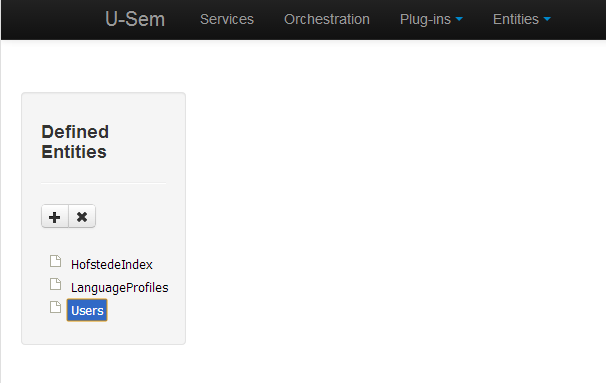
\includegraphics[scale=0.5]{ui/entityList.png}
  \caption{Context diagram of U-Sem }
  \label{fig_context}
\end{figure}
		
		\item \textbf{Entity manipulation panel} - The implementation also provide a panel that is responsible to automate the process of defining entities. Shown on figure \textbf{fig}, this panel is used when an entity is created or updated.
		
\begin{figure}[h!]
  \centering
  	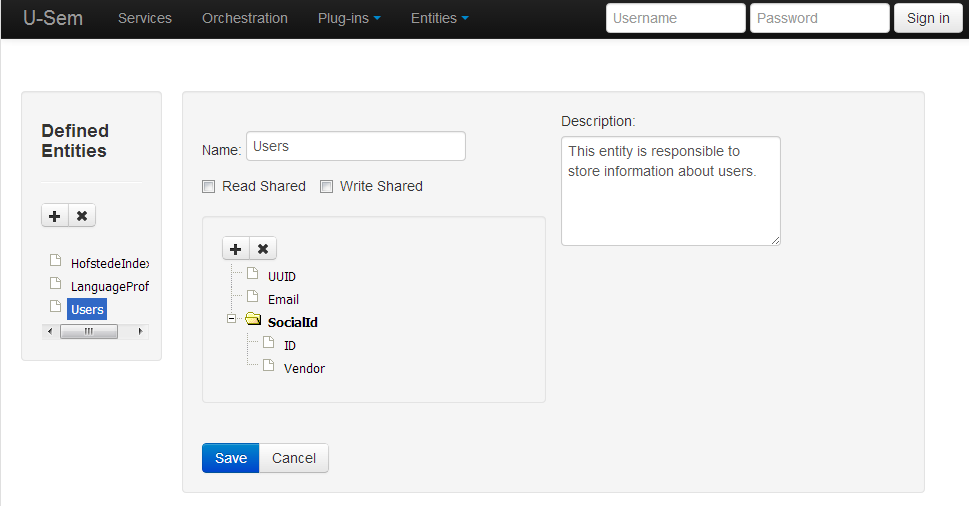
\includegraphics[scale=0.5]{ui/entityPanel.png}
  \caption{Context diagram of U-Sem }
  \label{fig_context}
\end{figure}

	\end{itemize}


\subsection{RDFGeards data manipulation components}
+ preview panel

input ports are set automatically to save time

\begin{figure}[h!]
  \centering
  	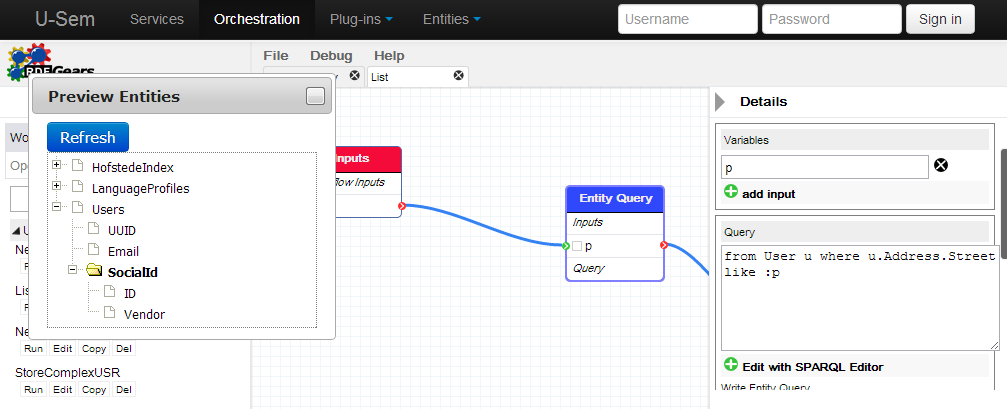
\includegraphics[scale=0.5]{ui/entityPreview.png}
  \caption{Context diagram of U-Sem }
  \label{fig_context}
\end{figure}

\subsection{Extended workflow compiler}

We implemented the extension of the capabilities by extending some of the classes involved in the feature and keeping the original classes intact. In this way, in case of problem or if needed engineers can easily switch between the two implementations. We extended the following classes:

\begin{itemize}
	\item \textit{WorkflowNode} - the newly created node is responsible to act as a wrapper around the output node of the workflow. When executed it triggers the execution of not only the output not but also to all the nodes with side effects defined in the workflow. The result of the execution is still the result of the execution of the output node. In this way we make sure that all nodes with side affects are executed as expected from the user. The already existing cashing mechanism enshures that each component is executed at most once which prevents any duplicate executions of components.
	
	\item \textit{WorkflowLoader} - the new child class extends the implementation in two directions. Firstly, when the workflow is compiled the resulted data structure contains not only the components needed for the execution of the output node but also the components with the side effects and their dependent components. Secondly, the output node implementations is replaced by the extended WorkflowNode, containing references to the output component and all components with side effects.
\end{itemize}


\section{Evaluation} 

After successfully implementing the system, in this section we evaluate whether the system complies with all functional and non-functional requirements defined at the beginning of this chapter.

\section{Limitations and Future work}

In this section we identify the limitations of the proposed architecture and we also suggest approaches that can be used to overcome these limitation in the future. We have identified the following items:

\begin{itemize}
\item One of the limitations that our approach introduces is the way semantics of data are defined. Currently, users can describe them only in text form(in the description field). The way entities are described is left to the engineer, there are no automated mechanisms that manage or assist the process. Therefore, more sophisticated (formal) approach for describing semantics of entities might be beneficial.

\item The aim of this feature is to simplify the work with persistent data in U-Sem. However, introducing this abstraction over the storage functionality we also have reduced the flexibility to some extend. One of the side effects is the inflexibility in terms of transactions management(begin, commit, rollback). In the current situation users do not have any means to manage the database transactions and they are tied to the way the engine is configured. Currently, our research showed that this is not a problem but in future some users might need to have the power to control the transactions to the database. Therefore, introducing a mechanism that can enable that efficiently might be an interesting research topic.

\item Most of the data manipulation components(except for the "Insert entity" component) require users to enter JPQL query. These queries can get quite complex and as a result users usually make some mistakes when writing them \textbf{cite}. Currently, the solution does not provide any facilities that can validate these queries. Users are notified abut the mistakes only when they try to execute the workflows and they fail. As a result, this process may cost a lot of time to users until they finally end up with the correct queries. Therefore, in future the system might be further improved by introducing functionality for autocomplition and validation of the JPQL queries.

\item \textbf{currently the engine does not guarantee the order of the execution of branches. Therefore, delevoping an mechanism to control the execution order can be really helpful}

\item Currently, the targeted to be used mainly as a research tool and there are no requirements for supporting large number of users and high loads. However, if the system is to be used in such demanding environment then it might be worth to research and improve the performance, scalability and availability properties of the solution. \textbf{maybe propose solutions like L2 cache and high availability db setups}. 

\end{itemize}

\begin{thebibliography}{99}

\bibitem{Neil} Object/Relational Mapping 2008: Hibernate and the Entity Data Model (EDM)

\bibitem{Hui} Supporting Database Applications as a Service

\bibitem{Feliksik} Eric Feliksik, RDF Gears, a data integration framework for the Semantic Web

\bibitem{Lu} Shiyong Lu, Jia Zhang, Collaborative Scientific Workflows, 2009

\bibitem{Lev} Y Lev, V Luchangco, M Olszewski, Scalable Reader-Writer Locks, 2009

\bibitem{terracotta} http://terracotta.org/

\bibitem{javadocs} http://docs.oracle.com/

\bibitem{Hernane} SL Hernane, J Gustedt, A Dynamic Distributed Algorithm for Read Write Locks . 2012

\end{thebibliography}

\end{document}